\chapter{Simulation Results}\label{cap:results}
This chapter presents the results achieved by the algorithms depicted in the Chapters \ref{cap:Swarm} and \ref{cap:contribution} using all optimization problems described in the Chapter \ref{cap:methodology}. This Chapter is divided in three parts:
\begin{itemize}
  \item A parametric analysis of the ABeePSO:
  \begin{itemize}
    \item Analysis of dispersion step;
    \item Analysis of acceleration coefficients ($c_1$ and $c_2$);
    \item Analysis of intervals of fuzzy membership functions;
    \item Analysis of stagnation counter;
  \end{itemize}
  \item Performance comparison among ABeePSO, PSO, APSO and ABC:
  \begin{itemize}
    \item Analysis of convergence;
    \item Analysis of the dimensionality;
    %\item Analysis of the diversity;
  \end{itemize}
  \item Initial analysis of the ClanABeePSO algorithm.
\end{itemize}

\section{Parametric Analysis of the ABeePSO}
This section presents the parametric analysis for the ABeePSO algorithm. This analysis aims to adapt the new operator and avoid explosion states in the ABeePSO algorithm. In this analysis, the number of dimensions is equal to 100 and the number of iterations is 1,000. All results were obtained over 10 trials.

\subsection{Analysis of Dispersion Step}
This analysis aims to investigate the influence of the parameters $\alpha$ and $\beta$ used to calculate the dispersion step of the guide bees (observe the Equation (\ref{eq:ABeePSO_Step})). We use one unimodal function ($F1$) and one multimodal function ($F16$). We selected a logistic function since we aim to have a step value around 1.0 for low $f_{evol}$ values and low step values for high $f_{evol}$ values.

We varied the value of $\alpha$ between 0 and 100, for $\beta$ = 0.1, 0.2 and 0.5. According to Figure \ref{fig:Dispersion_Step}, we observed that the best results were obtained for $\beta$ = 0.5. We also observed that the variation of $\alpha$ does not significantly interfere in the performance for the studied unimodal functions ($F1$) (Figure \ref{fig:Dispersion_F1}). In the multimodal function ($F16$), we observed that lower $\alpha$ values led to better results (Figure \ref{fig:Dispersion_F16}). Because of this, we assume $\alpha$ = 10.0 and $\beta$ = 0.5 for further simulations.

\begin{figure}[!h]
\centering
\subfigure[]{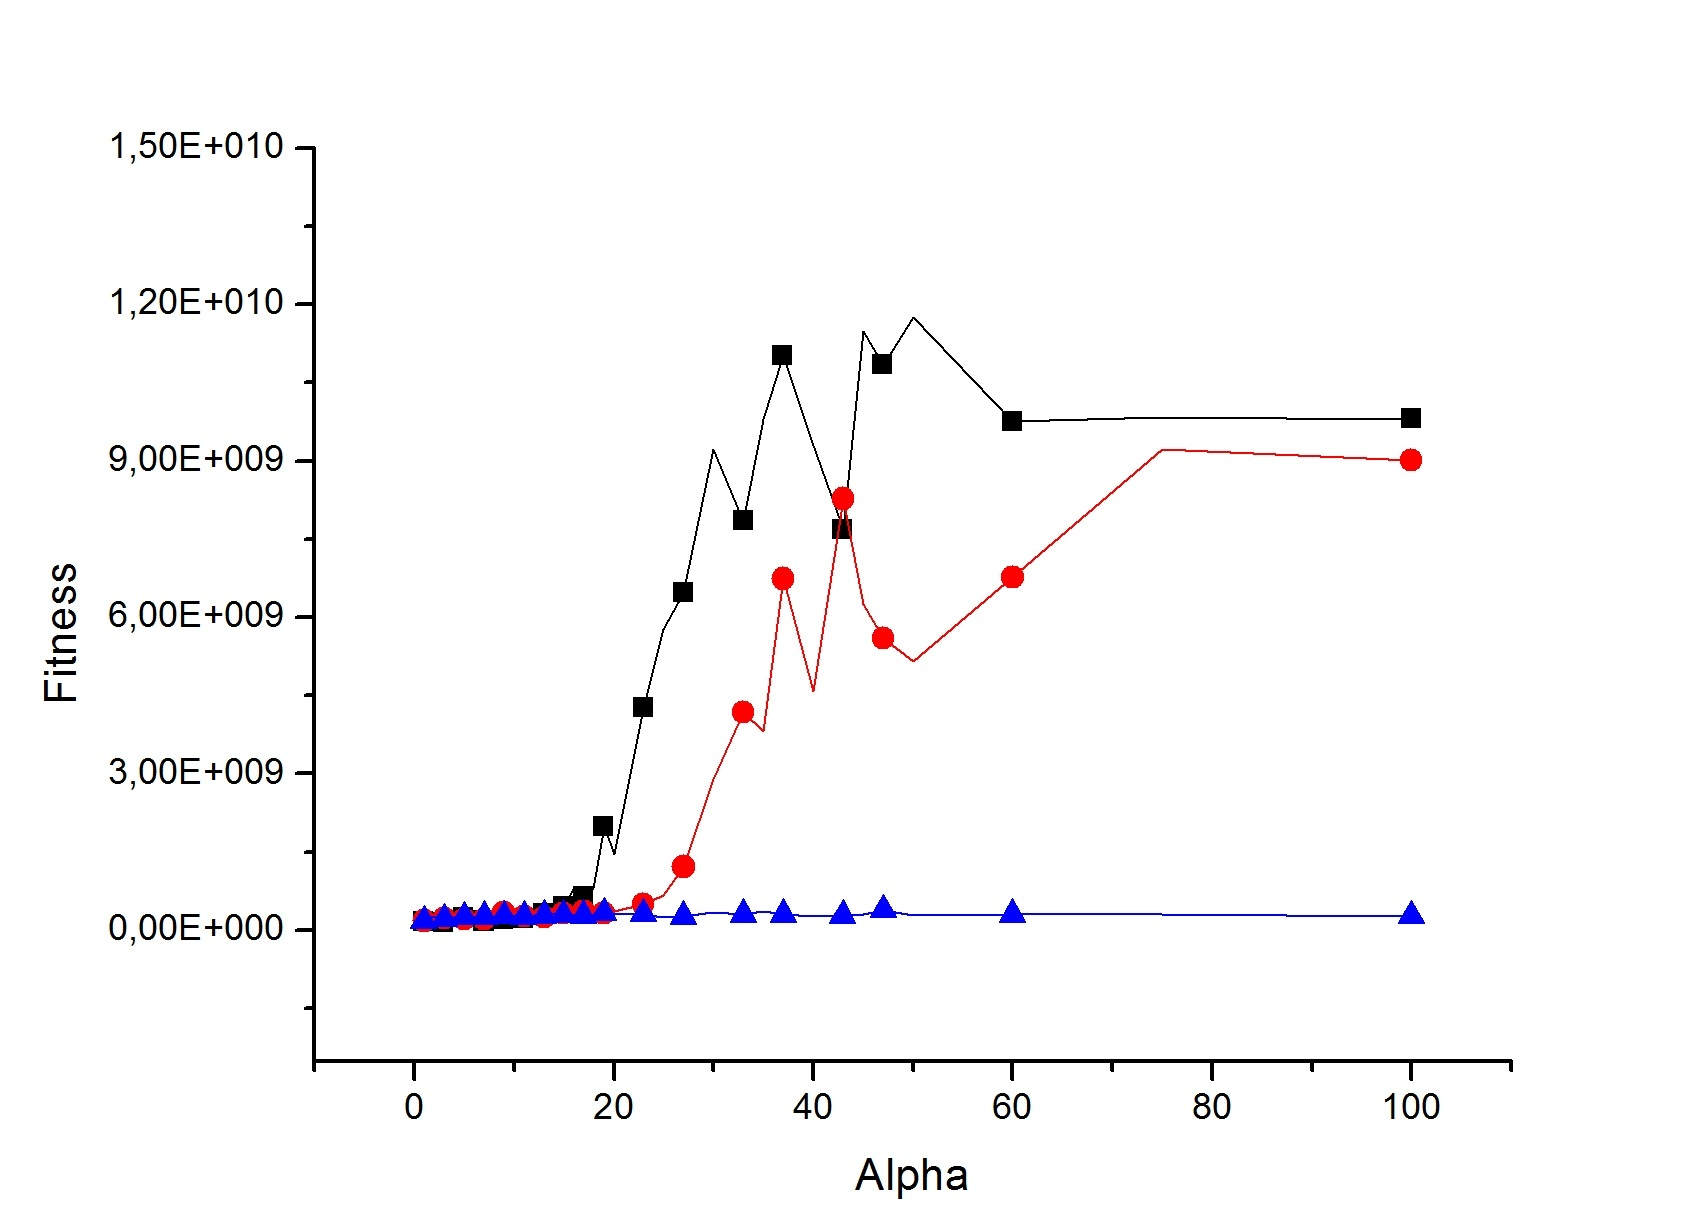
\includegraphics[scale=0.25]{results/dispersion/F1}\label{fig:Dispersion_F1}}
\hspace{1mm}
\subfigure[]{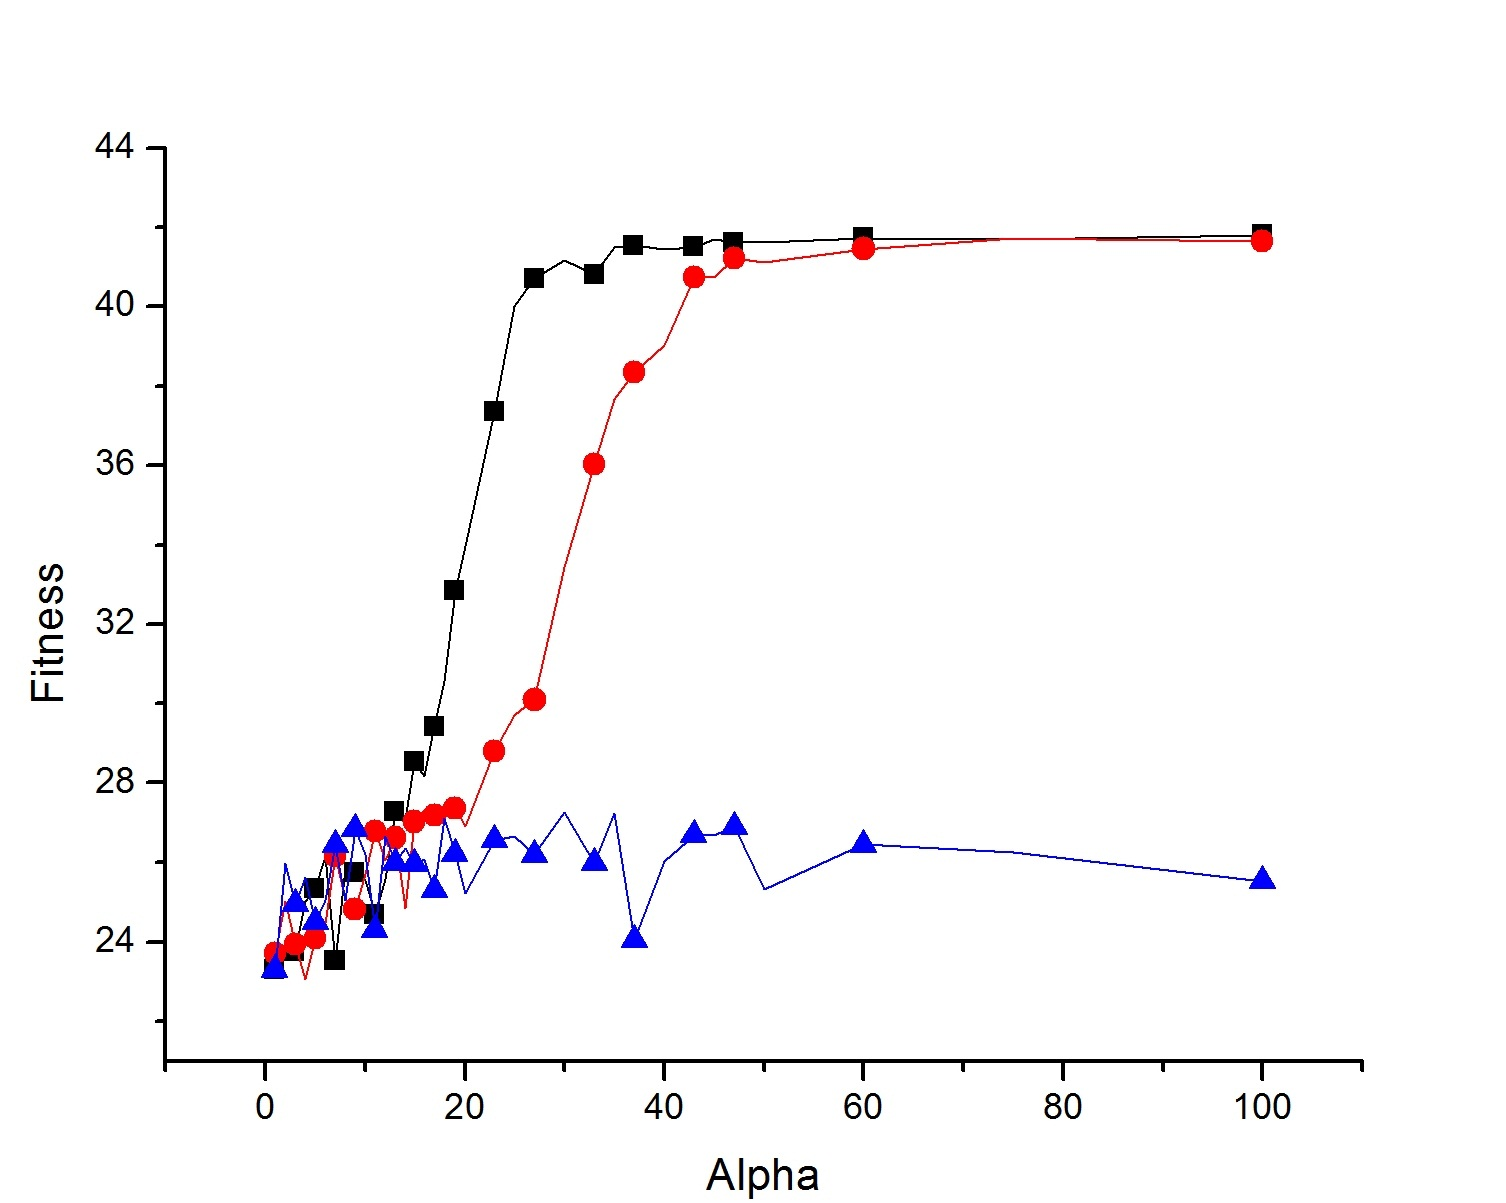
\includegraphics[scale=0.25]{results/dispersion/F16}\label{fig:Dispersion_F16}}
\caption{\small{Performance of the ABeePSO algorithm as a function of $\alpha$ for (a) $F1$ and (b) $F16$, considering $\beta$ = 0.1 (squares), $\beta$ = 0.2 (circles) and $\beta$ = 0.5 (triangle).}}
\label{fig:Dispersion_Step}
\end{figure}

\subsection{Analysis of Acceleration Coefficients ($c_1$ and $c_2$)}
Since the acceleration coefficients ($c_1$ and $c_2$) must be updated at each iteration and our proposal presents a different dynamic behavior, it is necessary to analyze the impact of the variation rate of $c_1$ and $c_2$ on the performance of our proposal. $\delta$ defines the increment (or decrement) of $c_1$ and $c_2$ per iteration. As lightly increment (or decrement) is performed by using $\delta/2$.

Table \ref{tab:acceleration_coefficients} shows the average fitness value for the functions $F4$ (unimodal) and $F13$ (multimodal) for different policies to determine $\delta$. The influence on the performance is not significant for the unimodal function, but the best result was achieved for a $\delta$ = 0.2. For the multimodal ($F13$), we the best results where achieved when $\delta$ is randomly chosen from the intervals $[0.01;0.05]$ and $[0.05;0.1]$. Since the difference between the results is not significant, we chose the same interval defined in the original APSO for further simulations, \textit{i.e.} $\delta$ randomly chosen from the interval $[0.05;0.1]$.

\begin{table}[!h]
\caption{\small{Impact of variation of acceleration rate in quality of search.}}
\centering
\begin{tabular}{c c c}
\hline
Value of $\delta$  &   $F4$               &  $F13$ \\
\hline
Random [0.01;0.1]    & 1.23E+14          & 1.02E+08 \\
Random [0.01;0.05]   & 1.33E+14          & \textbf{5.26E+07} \\
Random [0.02;0.1]    & 1.21E+14          & 5.91E+07 \\
Random [0.02;0.2]    & 1.38E+14          & 8.42E+07  \\
Random [0.05;0.1]    & 1.32E+14          & 5.72E+07  \\
Random [0.05;0.2]    & 1.37E+14          & 5.82E+07  \\
Fixed at 0.1          & 1.30E+14          & 8.91E+07  \\
Fixed at 0.2          & \textbf{1.13E+14} & 6.56E+07  \\
Fixed at 0.05         & 1.32E+14          & 1.05E+08  \\
\hline
\end{tabular}
\label{tab:acceleration_coefficients}
\end{table}

\subsection{Analysis of Intervals of Fuzzy Membership Functions}
This analysis is important since it determines the shift between APSO and ABeePSO. We performed some simulations for the functions $F4$ (unimodal) and $F13$ (multimodal) for different Fuzzy membership functions. The configuration 1 uses the Fuzzy membership functions depicted in Figure \ref{fig:factor_ABeePSO}. In the configuration 2 we modified the interval of the \emph{Convergence} state from 0.2 to 0.3 and the threshold of the \emph{Exploitation} state from 0.1 to 0.2, as one can observe in Figure \ref{fig:factor_ABeePSO_Test1}. This variation allows the algorithm to anticipate the start of the execution of the ABC based operator. In the configuration 3 we modified the interval of \emph{Exploitation} state from 0.5 to 0.6 and the threshold of the \emph{Exploration} state from 0.4 to 0.5, one can observe Figure \ref{fig:factor_ABeePSO_Test2}. This variation allows the execution of the ABC based operator for a longer time.

\begin{figure}[!h]
\centering
\subfigure[]{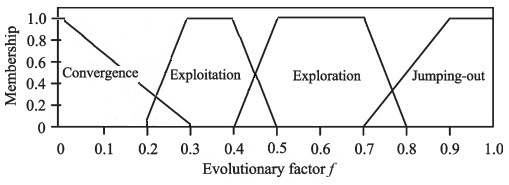
\includegraphics[scale=0.55]{results/fuzzy/factor_ABPSO_Test1.jpg}\label{fig:factor_ABeePSO_Test1}}
\hspace{1mm}
\subfigure[]{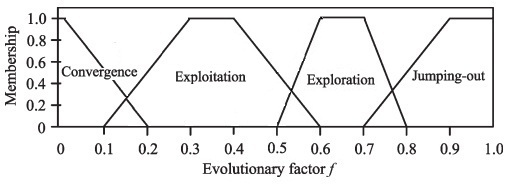
\includegraphics[scale=0.55]{results/fuzzy/factor_ABPSO_Test2.jpg}\label{fig:factor_ABeePSO_Test2}}
\caption{\small{Different configurations to analysis of intervals of fuzzy membership functions: (a) Configuration 2 and (b) Configuration 3.}}
\label{fig:Analysis_Fuzzy}
\end{figure}

For the unimodal function ($F7$), the configurations 1, 2 and 3 achieved average fitness (standard deviation) equal to $4.2E+10(8.53E+09)$, $4.59E+10(5.43E+09)$ and $4.9E+10(1.31E+09)$, respectively. For the multimodal function ($F20$), the configurations 1, 2 and 3 achieved the following average fitness (standard deviation) equal to $8.23E+08(2.5E+08)$, $1.02E+09(6.39E+08)$ and $1.29E+09(4.6E+08)$, respectively. The results indicate the configuration depicted in Figure \ref{fig:factor_ABeePSO}, \textit{i.e.} configuration 1. In other benchmark functions we observed that the dependence on the fuzzy intervals is higher for the multimodal functions, but the configuration depicted in Figure \ref{fig:factor_ABeePSO} is still the best option.

\subsection{Analysis of Stagnation Counter}
This initial analysis aims to estimate the initial value for stagnation counter and evaluate the behavior of algorithm with this information. We used one unimodal functions ($F4$) and multimodal function ($F2$).

We varied the value of stagnation counter is ranging between 0 and 100. According to results, we observed a similar performance for both functions. For the multimodal function, when the stagnation counter value is medium or high, the fitness value does not improve, \textit{i.e.} it is necessary to expand the swarm by using the ABC based operator and generate diversity. For the unimodal function, the best results were obtained when the stagnation counter value is low or medium. When the value is very high, the obtained fitness is mitigated. From this analysis, we defined a initial value equal 10.0 for stagnation step.

%\begin{figure}[!h]
%\centering
%\subfigure[]{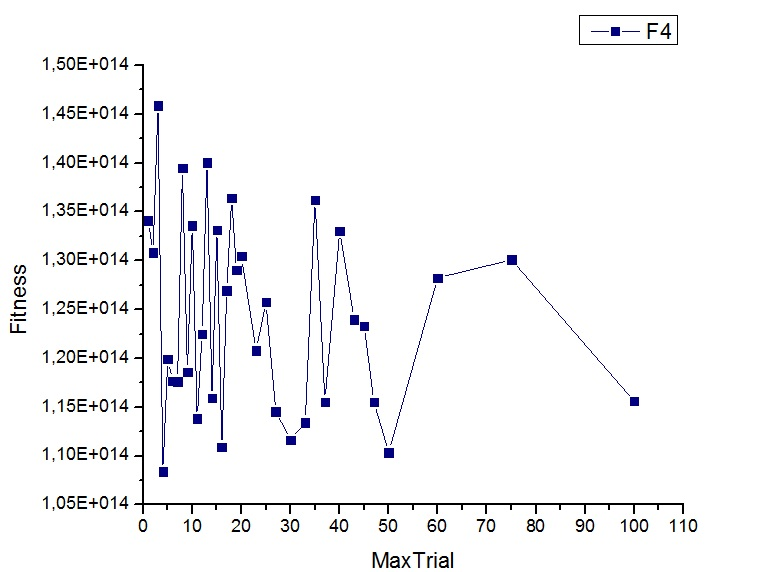
\includegraphics[scale=0.35]{results/stagnation/F4.jpg}\label{fig:Stagnation_F4}}
%\hspace{1mm}
%\subfigure[]{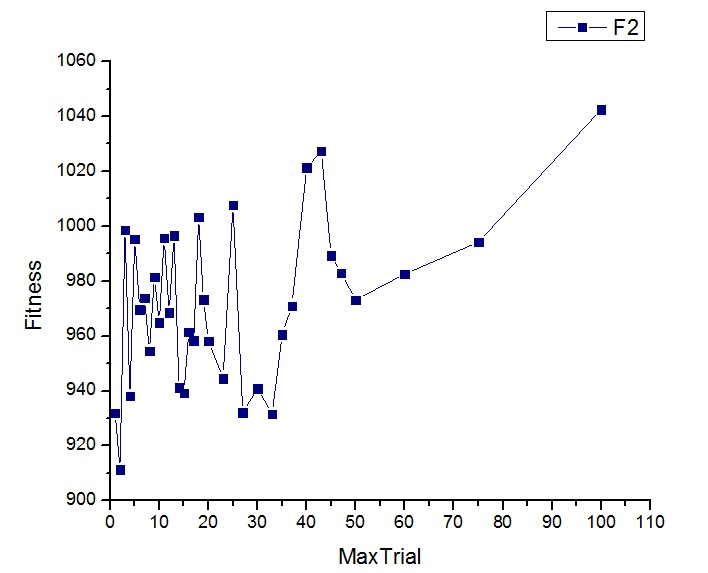
\includegraphics[scale=0.35]{results/stagnation/F2.jpg}\label{fig:Stagnation_F2}}
%\caption{\small{Performance of the ABPSO algorithm varying the value of stagnation counter in: (a) $F4$ and (b) $F2$.}}
%\label{fig:Stagnation}
%\end{figure}

\section{Performance comparison among ABeePSO, PSO, APSO and ABC}
This section presents a performance analysis of the ABeePSO algorithm and a comparison to the  PSO, APSO and ABC algorithms. We assessed the convergence velocity and scalability.
In the analysis of convergence, the number of dimensions is equal to 100 and the number of iterations is equal to 1,000. In the analysis of dimensionality, we performed 3,000, 5,000 and 10,000 iterations for 300, 500 and 1,000 dimensions, respectively. All results were obtained over 50 trials.
 %and the diversity analysis over 10 trials.

\subsection{Analysis of Convergence}
We compared the performance of various algorithms along the iterations to analyze the convergence velocity. Figure \ref{fig:Convergence} depicts the evolution of ABC, APSO PSO and ABeePSO algorithms for multimodal and unimodal benchmark functions. The Figures \ref{fig:Convergence_F3} and \ref{fig:Convergence_F5} are multimodal functions F3 and F5, respectively and Figures \ref{fig:Convergence_F12} and \ref{fig:Convergence_F14} are unimodal functions F12 and F14, respectively. We did not observe a significant improvement in the convergence velocity for unimodal function. However, our proposal outperformed the other approaches for the multimodal problems, mainly for the F3 function.

\begin{figure}[!h]
\centering
\subfigure[]{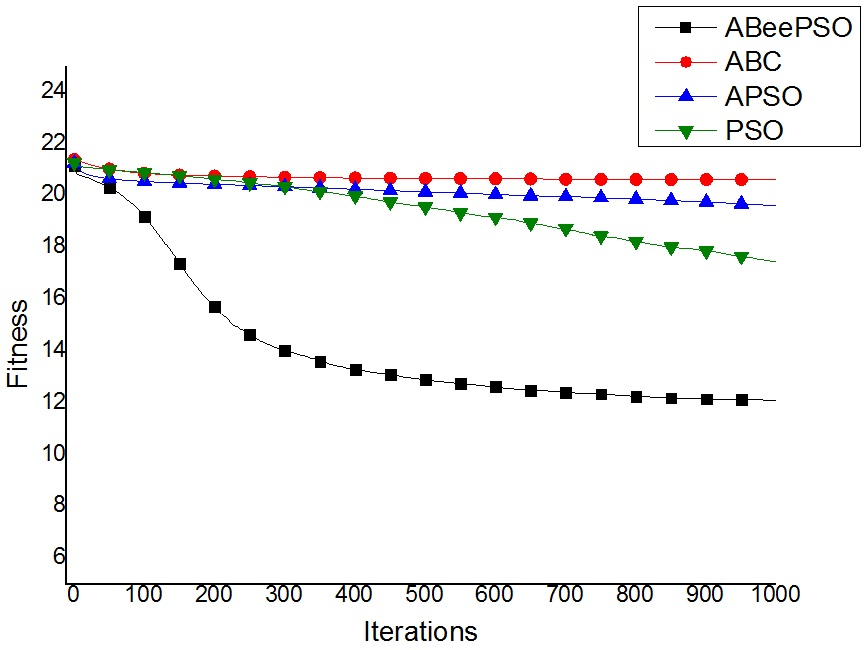
\includegraphics[scale=0.22]{results/convergence/F3}\label{fig:Convergence_F3}}
\hspace{1mm}
\subfigure[]{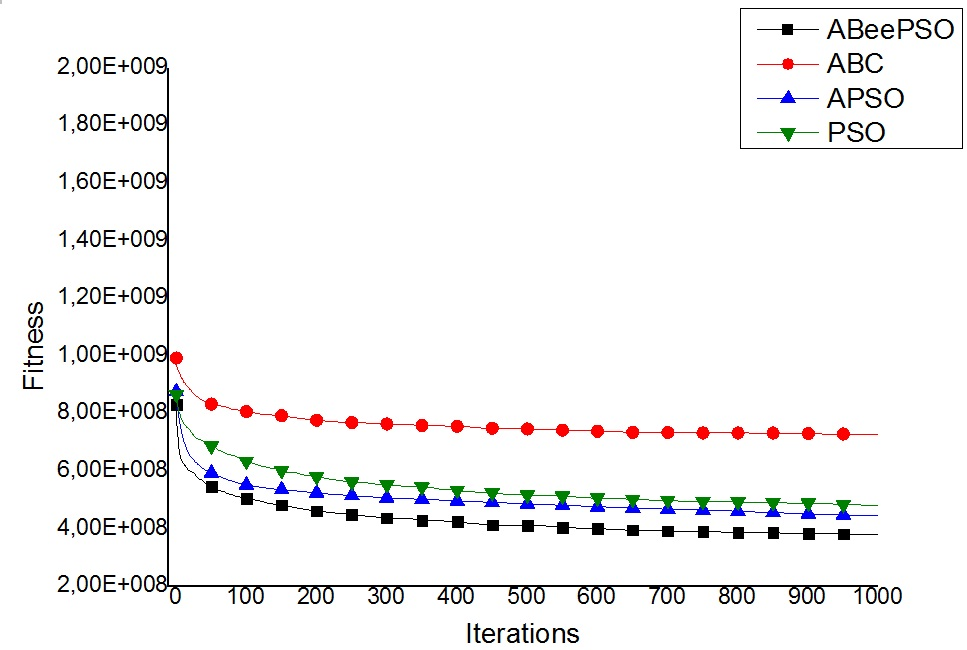
\includegraphics[scale=0.22]{results/convergence/F5}\label{fig:Convergence_F5}}
\hspace{1mm}
\subfigure[]{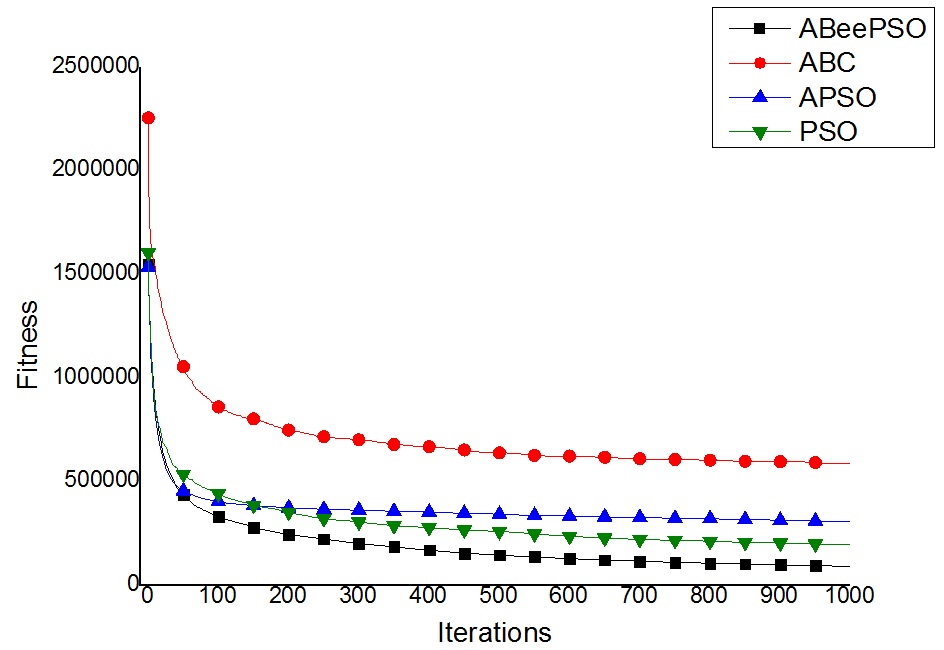
\includegraphics[scale=0.22]{results/convergence/F12}\label{fig:Convergence_F12}}
\hspace{1mm}
\subfigure[]{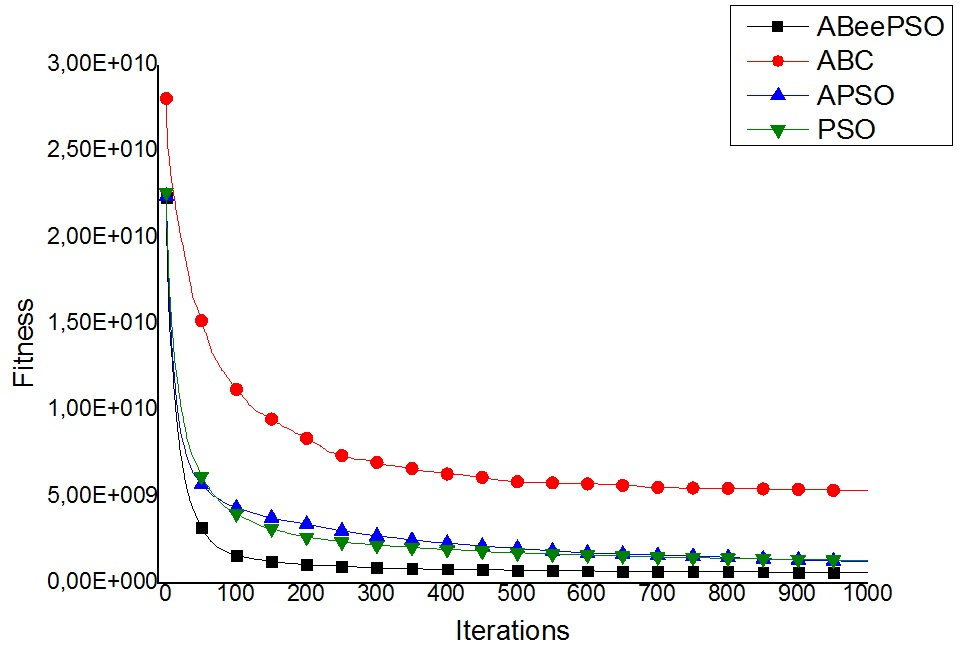
\includegraphics[scale=0.22]{results/convergence/F14}\label{fig:Convergence_F14}}
\caption{\small{Analysis of Convergence: Fitness function evolution of the ABC, APSO, PSO and ABeePSO algorithms for the $D$ = 100 in (a) $F3$, (b) $F5$, (c) $F12$ and (d) $F14$ functions.}}
\label{fig:Convergence}
\end{figure}

\subsection{Analysis of Scalability}
We also analyzed the performance of the algorithms as a function of the number of dimensions of the problem. We aim to analyze the scalability of the algorithms. As the dimensionality increases, the difficulty of the problems also increases. Figures \ref{fig:Dimensionality_F7} and \ref{fig:Dimensionality_F11} show the boxplot of the fitness as a function of the dimensionality for the benchmark functions $F7$ (unimodal) and $F11$ (multimodal), respectively.

For the unimodal function, one can observe that the ratio between the performance of the algorithms is maintained, but it is smaller for $D$ = 1,000.

For the multimodal function, we obtained better results when compared to other approaches, \textit{i.e.} the difference in the performance between our proposal and other techniques is maintained as the dimensionality of the problem also increases.

\begin{figure}[!h]
\centering
\subfigure[]{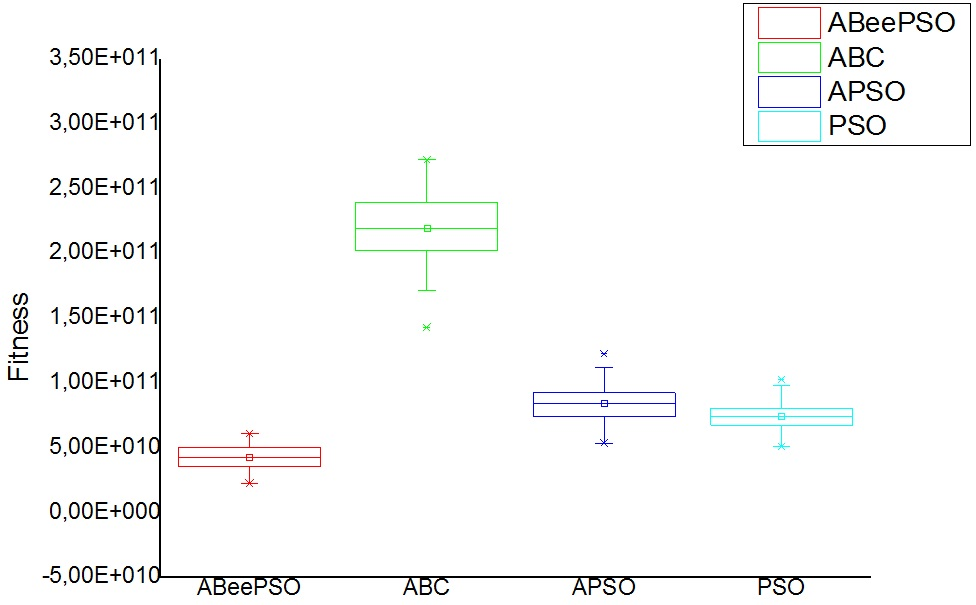
\includegraphics[scale=0.22]{results/dimensionality/F7-100D}\label{fig:Dimensionality_F7_100D}}
\hspace{1mm}
\subfigure[]{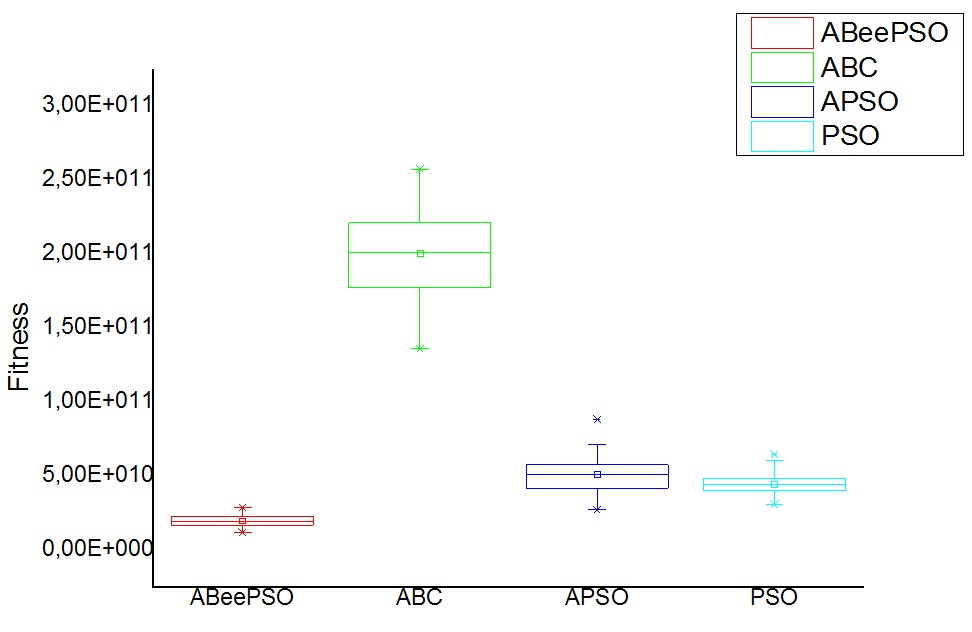
\includegraphics[scale=0.22]{results/dimensionality/F7-300D}\label{fig:Dimensionality_F7_300D}}
\hspace{1mm}
\subfigure[]{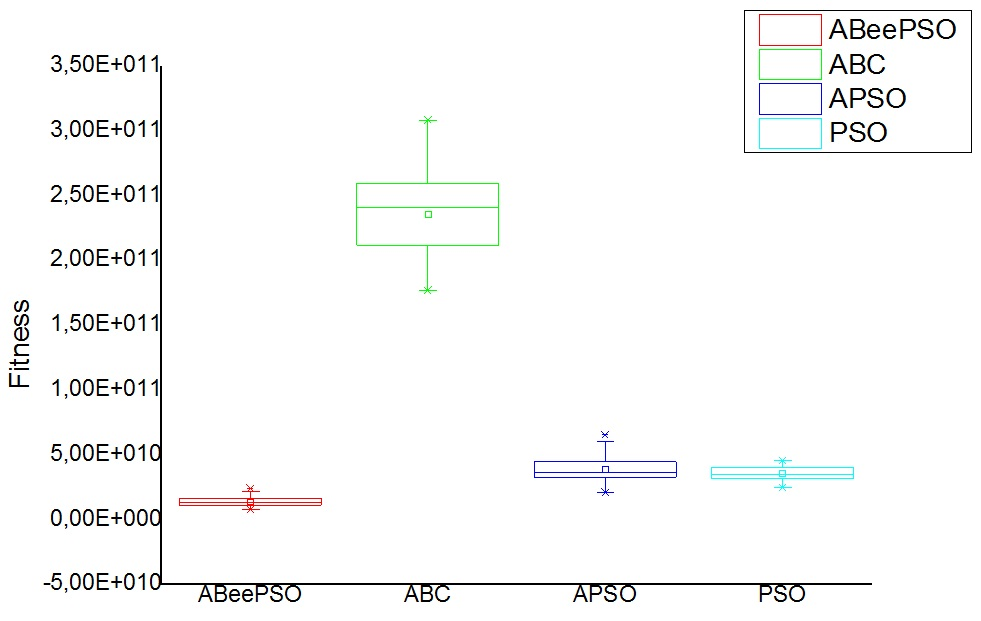
\includegraphics[scale=0.22]{results/dimensionality/F7-500D}\label{fig:Dimensionality_F7_500D}}
\hspace{1mm}
\subfigure[]{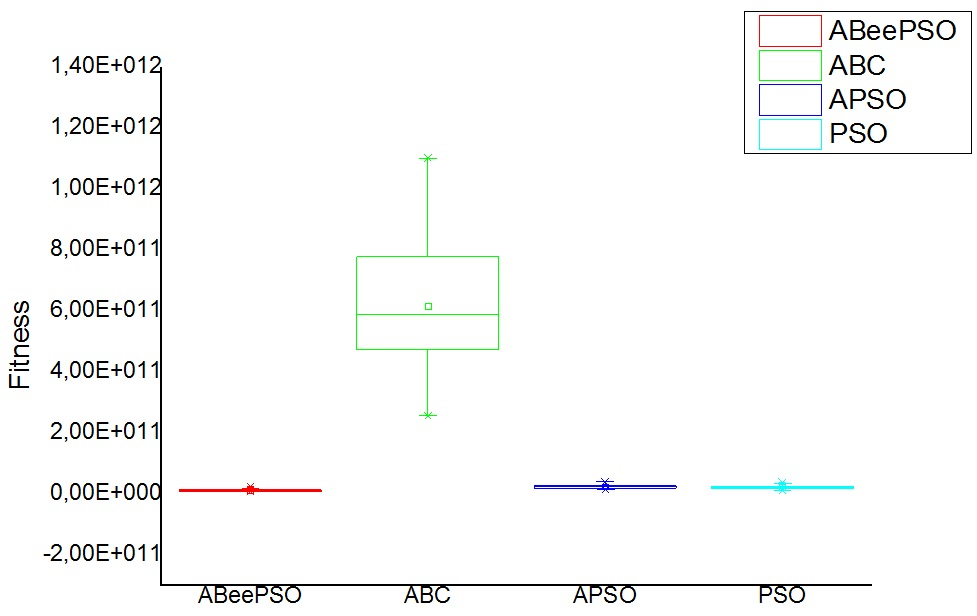
\includegraphics[scale=0.22]{results/dimensionality/F7-1000D}\label{fig:Dimensionality_F7_1000D}}
\caption{\small{Analysis of the Dimensionality: Boxplot of the fitness for the $F7$ function varying the number of dimensions for (a) $D$ = 100, (b) $D$ = 300, (c) $D$ = 500 and (d) $D$ = 1,000.}}
\label{fig:Dimensionality_F7}
\end{figure}

\begin{figure}[!h]
\centering
\subfigure[]{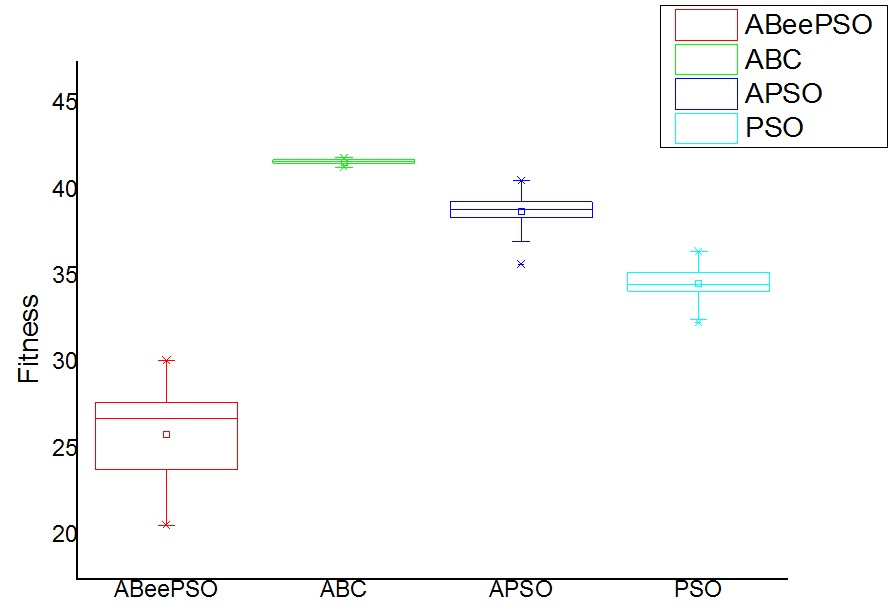
\includegraphics[scale=0.22]{results/dimensionality/F11-100D}\label{fig:Dimensionality_F11_100D}}
\hspace{1mm}
\subfigure[]{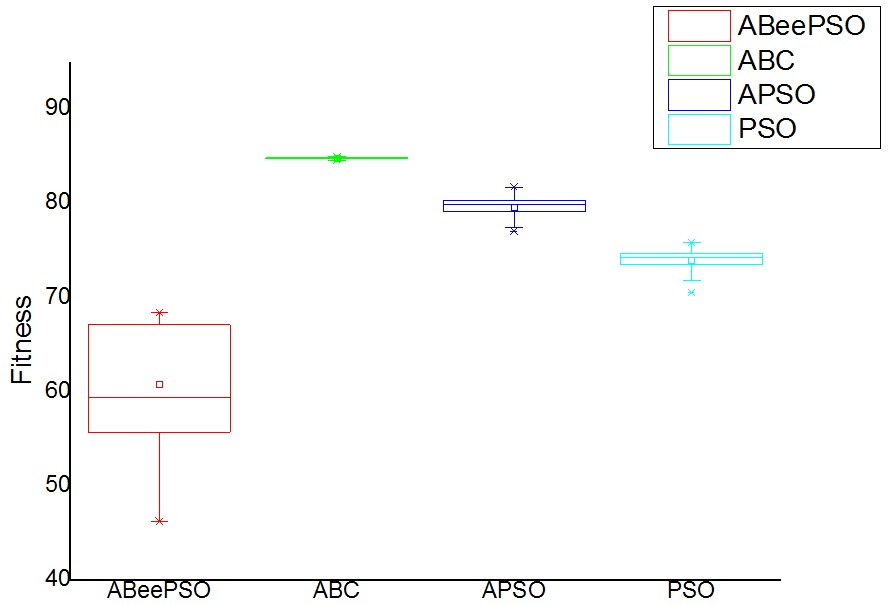
\includegraphics[scale=0.22]{results/dimensionality/F11-300D}\label{fig:Dimensionality_F11_300D}}
\hspace{1mm}
\subfigure[]{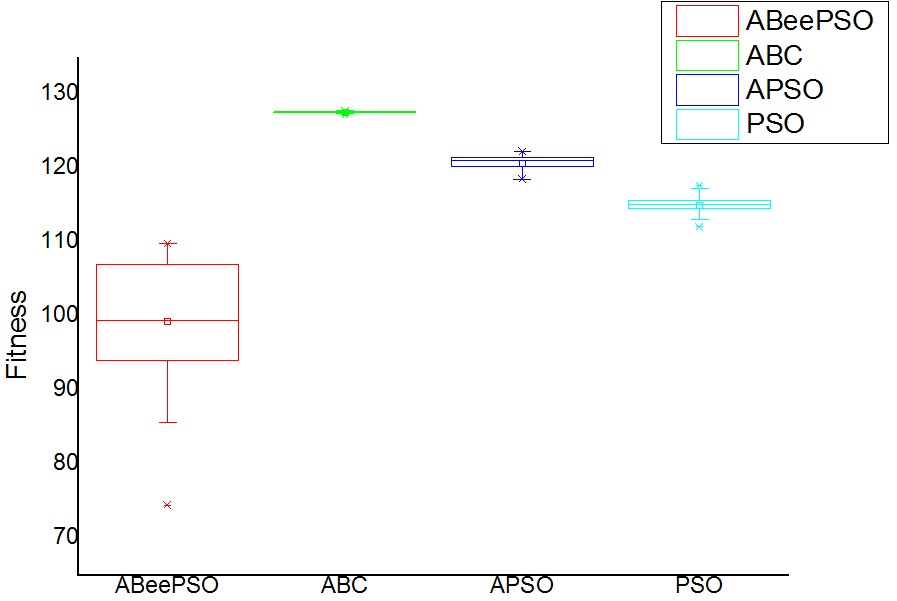
\includegraphics[scale=0.22]{results/dimensionality/F11-500D}\label{fig:Dimensionality_F11_500D}}
\hspace{1mm}
\subfigure[]{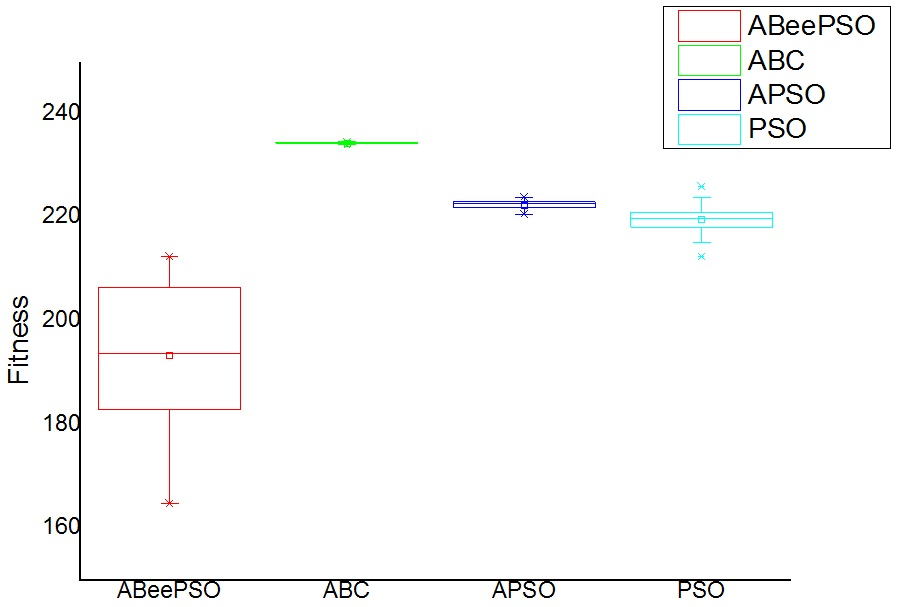
\includegraphics[scale=0.22]{results/dimensionality/F11-1000D}\label{fig:Dimensionality_F11_1000D}}
\caption{\small{Analysis of the Dimensionality: Boxplot of the fitness for the $F11$ function varying the number of dimensions for (a) $D$ = 100, (b) $D$ = 300, (c) $D$ = 500 and (d) $D$ = 1,000.}}
\label{fig:Dimensionality_F11}
\end{figure}

We realized experiments with all benchmark functions, varying the number of dimensions. We made the comparison the ABeePSO with ABC, APSO and PSO algorithms. Tables \ref{tab:Comparison_100D}, \ref{tab:Comparison_300D}, \ref{tab:Comparison_500D} and \ref{tab:Comparison_1000D} present the average fitness and (standard deviation) obtained from simulations for 100, 300, 500 and 1,000 dimensions, respectively. The best average fitness values is highlighted for each benchmark function.

\begin{table}[!h]
\caption{\small{Performance comparison in terms of average fitness value and (standard deviation) between ABeePSO, PSO, APSO and ABC for all the 20 benchmark functions for 100 dimensions.}}
\label{tab:Comparison_100D}
\begin{center}
\begin{tabular}{p{0.5cm}|p{2.5cm}|p{2.5cm}|p{2.5cm}|p{2.5cm}}
\hline\noalign{\smallskip}
\textbf{F\#}	& ABeePSO & ABC & APSO & PSO    \\		
\noalign{\smallskip}
\hline
\noalign{\smallskip}
\textit{F1}  & \textbf{2.86E+08 (8.22E+07)} & 9.20E+09 (1.92E+09) & 3.23E+09 (1.19E+09) & 9.16E+08 (1.62E+08)\\
\textit{F2}  & 9.58E+02 (63.09667) & 1.31E+03 (85.5529) & \textbf{9.10E+02 (70.90304)} & 1.21E+03 (62.80075)\\
\textit{F3}  & \textbf{12.07975 (0.656529)} & 20.62107 (0.08368) & 19.62592 (0.401446) & 17.45967 (0.635132)\\
\textit{F4}  & \textbf{1.32E+14 (3.05E+13)} & 1.58E+15 (3.05E+14) & 3.11E+14 (1.24E+14) & 2.84E+14 (5.87E+13)\\
\textit{F5}  & \textbf{3.81E+08 (2.64E+07)} & 7.28E+08 (3.32E+07) & 4.45E+08 (4.70E+07) & 4.81E+08 (2.75E+07)\\
\textit{F6}  & \textbf{7.59E+06 (8.71E+05)} & 2.09E+07 (6.01E+04) & 1.97E+07 (3.27E+05) & 1.28E+07 (6.37E+05)\\
\textit{F7}  & \textbf{4.33E+10 (9.10E+09)} & 2.19E+11 (2.79E+10) & 8.45E+10 (1.61E+10) & 7.50E+10 (1.2E+10)\\
\textit{F8}  & \textbf{6.78E+13 (5.49E+05)} & 7.98E+16 (2.01E+16) & 2.99E+16 (9.34E+15) & 4.49E+14 (1.19E+14)\\
\textit{F9}  & \textbf{4.02E+08 (9.68E+07)} & 2.16E+09 (6.70E+08) & 1.15E+09 (4.64E+08) & 1.11E+09 (1.52E+08)\\
\textit{F10} & 9.73E+02 (39.83971) & 1.64E+03 (68.497) & \textbf{8.54E+02 (77.301)} & 1.23E+03 (64.016)\\
\textit{F11} & \textbf{25.93234 (2.34576)} & 41.67951 (0.132561) & 38.83987 (0.875927) & 34.68351 (0.87051)\\
\textit{F12} & \textbf{9.26E+04 (1.67E+04)} & 5.86E+05 (7.60E+04) & 3.08E+05 (5.03E+04) & 1.95E+05 (2.19E+04)\\
\textit{F13} & \textbf{8.08E+07 (7.19E+07)} & 6.46E+10 (1.52E+10) & 2.00E+10 (5.99E+09) & 4.69E+08 (1.19E+08)\\
\textit{F14} & \textbf{6.29E+08 (1.21E+08)} & 5.36E+09 (9.68E+08) & 1.26E+09 (3.63E+08) & 1.32E+09 (2.21E+08)\\
\textit{F15} & \textbf{9.82E+02 (40.05412)} & 1.75E+03 (57.49683) & 1.15E+03 (62.5245) & 1.24E+03 (67.00242)\\
\textit{F16} & \textbf{25.48114 (2.66121)} & 42.02208 (0.098697) & 40.38697 (0.411129) & 35.10031 (0.811823)\\
\textit{F17} & \textbf{1.84E+05 (2.29E+04)} & 6.79E+05 (7.42E+04) & 3.04E+05 (3.85E+04) & 2.77E+05 (3.40E+04)\\
\textit{F18} & \textbf{1.02E+09 (6.82E+08)} & 2.01E+11 (3.15E+10) & 8.16E+10 (1.37E+10) & 1.16E+10 (3.25E+09)\\
\textit{F19} & \textbf{2.09E+05 (2.82E+04)} & 8.01E+05 (7.82E+04) & 4.03E+05 (9.40E+04) & 3,08E+05 (3.96E+04)\\
\textit{F20} & \textbf{1.09E+09 (6.41E+08)} & 2.58E+11 (4.56E+10) & 1.12E+11 (1.81E+10) & 1.17E+10 (5.35E+09)\\
\hline
\end{tabular}
\end{center}
\end{table}

\begin{table}[!h]
\caption{\small{Performance comparison in terms of average fitness value and (standard deviation) between ABeePSO, PSO, APSO and ABC for all the 20 benchmark functions for 300 dimensions.}}
\label{tab:Comparison_300D}
\begin{center}
\begin{tabular}{p{0.5cm}|p{2.5cm}|p{2.5cm}|p{2.5cm}|p{2.5cm}}
\hline\noalign{\smallskip}
\textbf{F\#}	& ABeePSO & ABC & APSO & PSO    \\		
\noalign{\smallskip}
\hline
\noalign{\smallskip}
\textit{F1}	& \textbf{1.41E+09 (2.11E+08)} & 6.12E+10 (4.48E+09) & 1.41E+09 (1.2E+09) & 6.14E+09 (7.23E+08) \\
\textit{F2}	& 4.03E+03 (1.52E+02) & 5.40E+03 (1.43E+02) & \textbf{1.53E+03 (1.27E+02)} & 4.39E+03 (1.26E+02)\\		
\textit{F3}	& \textbf{13.81304 (0.40062)} & 21.04023 (0.041704) & 17.86329 (0.629742) & 20.49093 (0.160888) \\
\textit{F4}& \textbf{5.88E+13 (1.64E+13)} & 2.44E+15 (5.44E+14) & 9.07E+13 (4.39E+13) & 1.62E+14 (3.97E+13) \\
\textit{F5}& \textbf{3.29E+08 (3.68E+07)} & 8.14E+08 (3.59E+07) & 4.08E+08 (4.82E+07) & 4.11E+08 (2.45E+07) \\
\textit{F6}& \textbf{4.81E+06 (3.94E+05)} & 2.08E+07 (9.46E+04) & 1.91E+07 (3.26E+05) & 9.62E+06 (5.56E+05) \\
\textit{F7}& \textbf{2.03E+10 (4.10E+09)} & 2.01E+11 (2.92E+10) & 5.16E+10 (1.19E+10) & 4.51E+10 (6.51E+09) \\
\textit{F8}& \textbf{3.13E+13 (9.01E+12)} & 6.78E+16 (1.56E+16) & 1.79E+16 (8.31E+15) & 6.3E+13 (1.75E+13) \\
\textit{F9}& \textbf{2.42E+09 (3.48E+08)} & 6.09E+10 (5.72E+09) & 3.18E+09 (2.02E+09) & 6.66E+09 (7.21E+08) \\
\textit{F10}& \textbf{8.50E+02 (3.96E+01)} & 6.06E+03 (1.27E+02) & 2.65E+03 (1.30E+02) & 4.59E+03 (1.12E+02)\\
\textit{F11}& \textbf{60.82139 (6.383927)} & 84.81496 (0.08274) & 79.68142 (1.100449) & 74.01696 (1.241357) \\
\textit{F12}& \textbf{6.02E+05 (4.74E+04)} & 2.31E+06 (1.70E+05) & 7.39E+05 (9.22E+04) & 1.06E+06 (5.85E+04)\\
\textit{F13}& \textbf{4.14E+08 (9.32E+07)} & 6.71E+11 (5.86E+10) & 1.07E+11 (3.14E+10) & 9.34E+09 (2.64E+09)\\
\textit{F14}& \textbf{2.39E+09 (2.57E+08)} & 3.96E+10 (5.34E+09) & 2.50E+09 (3.30E+08) & 7.28E+09 (7.06E+08)\\
\textit{F15}& 4.01E+03 (1.42E+02) & 6.00E+03 (1.18E+02) & \textbf{3.16E+03 (1.47E+02)} & 4.49E+03 (1.04E+02)\\
\textit{F16}& \textbf{96.59136 (7.406842)} & 127.2318 (0.128599) & 123.3011 (0.418354) & 118.5161 (1.745353)\\
\textit{F17}& \textbf{8.41E+05 (8.24E+04)} & 4.76E+06 (6.23E+05) & 9.26E+05 (1.04E+04) & 1.45E+06 (1.59E+05)\\
\textit{F18}& \textbf{4.23E+09 (1.39E+09)} & 1.35E+12 (1.01E+11) & 7.53E+10 (5.31E+10) & 4.70E+12 (8.02E+10)\\
\textit{F19}& 1.37E+06 (1.35E+05) & 6.82E+06 (7.44E+05) & \textbf{1.30E+06 (3.48E+05)} & 2.11E+06 (2.41E+05)\\
 \textit{F20}& \textbf{6.04E+09 (2.87E+09)} & 1.51E+12 (1.18E+11) & 1.57E+11 (3.14E+10) & 1.78E+11 (2.19E+10)\\
\hline
\end{tabular}
\end{center}
\end{table}


\begin{table}[!h]
\caption{\small{Performance comparison in terms of average fitness value and (standard deviation) between ABeePSO, PSO, APSO and ABC for all the 20 benchmark functions for 500 dimensions.}}
\label{tab:Comparison_500D}
\begin{center}
\begin{tabular}{p{0.5cm}|p{2.5cm}|p{2.5cm}|p{2.5cm}|p{2.5cm}}
\hline\noalign{\smallskip}
\textbf{F\#}	& ABeePSO & ABC & APSO & PSO    \\		
\noalign{\smallskip}
\hline
\noalign{\smallskip}
\textit{F1}	& \textbf{2.17E+09 (3.24E+08)} & 1.22E+11 (7.33E+09) & 2.86E+09 (2.27E+09) & 1.19E+10 (8.12E+08)\\		
\textit{F2}	& 6.57E+03 (1.70E+02) & 9.91E+03 (2.04E+02) & \textbf{2.86E+03 (2.27E+02)} & 7.59E+03 (1.27E+02)\\		
\textit{F3}	& \textbf{14.58456 (0.524085)} & 21.17949 (0.043387) & 18.05753 (0.4994) & 20.77854 (0.058559) \\
\textit{F4} & \textbf{4.81E+13 (1.26E+13)} & 2.30E+15 (4.41E+14) & 6.83E+13 (2.67E+13) & 1.28E+14 (2.84E+13)\\		
\textit{F5} & \textbf{3.09E+08 (3.86E+07)} & 7.68E+08 (3.67E+07) & 3.42E+08 (4.52E+07) & 3.97E+08 (2.40E+07)\\
\textit{F6} & \textbf{4.47E+06 (5.79E+05)} & 2.09E+07 (9.32E+04) & 1.94E+07 (2.65E+05) & 8.73E+06 (3.13E+05)\\
\textit{F7} & \textbf{1.41E+10 (3.68E+09)} & 2.36E+11 (3.26E+10) & 3.91E+10 (9.61E+09) & 3.58E+10 (5.45E+09)\\
\textit{F8} & \textbf{9.43E+12 (2.90E+12)} & 1.22E+17 (1.88E+16) & 5.51E+15 (3.65E+15) & 2.64E+13 (8.72E+12)\\
\textit{F9} & 3.82E+09 (5.49E+08) & 1.25E+11 (9.68E+09) & \textbf{2.67E+09 (5.02E+08)} & 1.52E+10 (1.20E+09)\\
\textit{F10}& 7.20E+03 (1.90E+02) & 1.06E+04 (1.39E+02) & \textbf{4.21E+03 (1.48E+02)} & 7.87E+03 (1.34E+02)\\
\textit{F11}& \textbf{99.34556 (8.08220)} & 127.5809 (0.10924) & 120.7821 (0.91662) & 115.0733 (1.05427) \\
\textit{F12}& 1.13E+06 (6.99E+04) & 5.69E+06 (4.68E+05) & \textbf{8.53E+05 (8.87E+04)} & 2.05E+06 (1.11E+05)\\
\textit{F13}& \textbf{5.21E+08 (1.25E+08)} & 1.30E+12 (7.93E+10) & 1.67E+10 (1.10E+10) & 4.00E+10 (9.53E+09)\\
\textit{F14}& 4.37E+09 (4.61E+08) & 1.04E+11 (7.25E+09) & \textbf{3.89E+09 (2.89E+08)} & 1.55E+10 (1.00E+09)\\
\textit{F15}& 7.34E+03 (1.50E+02) & 1.07E+04 (1.13E+02) & \textbf{6.43E+03 (2.41E+02)} & 8.01E+03 (1.20E+02)\\
\textit{F16}& \textbf{166.3537 (9.092158)} & 212.7954 (0.119684) & 206.1731 (0.543216) & 205.4262 (1.845581)\\
\textit{F17}& \textbf{1.46E+06 (1.16E+05)} & 1.05E+07 (1.30E+06) & 1.73E+06 (1.16E+05) & 2.91E+06 (2.04E+05)\\
\textit{F18}& \textbf{1.38E+10 (2.01E+09)} & 2.77E+12 (1.59E+11) & 1.32E+11 (5.89E+10) & 3.48E+11 (2.90E+10)\\
\textit{F19}& 4.23E+06 (3.37E+05) & 1.75E+07 (1.98E+06) & \textbf{3.85E+06 (8.90E+05)} & 5.40E+06 (4.68E+05)\\
\textit{F20}& \textbf{1.43E+10 (2.20E+09)} & 3.03E+12 (1.39E+11) & 1.33E+11 (6.61E+10) & 4.24E+11 (3.70E+10)\\
\hline
\end{tabular}
\end{center}
\end{table}

\begin{table}[!h]
\caption{\small{Performance comparison in terms of average fitness value and (standard deviation) between ABeePSO, PSO, APSO and ABC for all the 20 benchmark functions for 1,000 dimensions.}}
\label{tab:Comparison_1000D}
\begin{center}
\begin{tabular}{p{0.5cm}|p{2.5cm}|p{2.5cm}|p{2.5cm}|p{2.5cm}}
\hline\noalign{\smallskip}
\textbf{F\#}	& ABeePSO & ABC & APSO & PSO    \\		
\noalign{\smallskip}
\hline
\noalign{\smallskip}
\textit{F1}	& \textbf{9.49E+09 (7.41E+08)} & 2.93E+11 (9.25E+09) & 1.02E+10 (4.10E+09) & 3.34E+10 (2.09E+09)\\		
\textit{F2}	& 14295.42 (305.095) & 21862.81 (414.0550) & \textbf{5646.419 (251.3274)} & 15878.37 (201.1898)\\		
\textit{F3}	& 20.5246 (0.2398) & 21.3259 (0.0189) & \textbf{18.2617 (0.3523)} & 20.9554 (0.0209)\\
\textit{F4} & \textbf{5.55E+13 (1.52E+13)} & 2.29E+15 (4.13E+14) & 6.37E+13 (2.35E+13) & 1.05E+14 (2.39E+13)\\		
\textit{F5} & \textbf{2.73E+08 (4.07E+07)} & 8.38E+08 (2.99E+07) & 3.42E+08 (4.52E+07) & 3.38E+08 (2.58E+07)\\
\textit{F6} & \textbf{1.36E+06 (3.81E+05)} & 2.08E+07 (9.16E+04) & 1.90E+07 (3.35E+05) & 6.41E+06 (4.34E+05)\\
\textit{F7} & \textbf{1.22E+10 (3.52E+09)} & 6.17E+11 (2.13E+11) & 2.51E+10 (6.68E+09) & 2.38E+10 (5.68E+09)\\
\textit{F8} & \textbf{3.34E+12 (1.14E+12)} & 9.58E+16 (1.49E+16) & 1.99E+15 (2.13E+15) & 6.62E+12 (2.83E+12)\\
\textit{F9} & 9.98E+09 (7.77E+08) & 3.07E+11 (1.43E+10) & \textbf{4.47E+09 (9.55E+08)} & 3.89E+10 (2.91E+09)\\
\textit{F10}& 15171.77 (225.8321) & 22536.49 (250.1126) & \textbf{8758.037 (234.3429)} & 16291.16 (223.1056)\\
\textit{F11}& \textbf{193.5644 (12.4481)} & 234.4677 (0.1527) & 222.5258 (0.7495) & 219.8308 (2.6664)\\
\textit{F12}& 3.80E+06 (2.05E+05) & 1.86E+07 (1.71E+06) & \textbf{1.71E+06 (1.55E+05)} & 4.76E+06 (2.12E+05)\\
\textit{F13}& \textbf{3.61E+09 (4.71E+08)} & 2.87E+12 (1.03E+11) & 2.87E+10 (1.24E+10) & 1.75E+11 (1.88E+10)\\
\textit{F14}& 1.22E+10 (3.52E+09) & 3.03E+11 (1.95E+10) & \textbf{7.41E+09 (5.23E+08)} & 4.09E+10 (2.52E+09)\\
\textit{F15}& 15229.42 (210.007) & 22634.39 (172.2981) & \textbf{12939.51 (253.0937)} & 16404.02 (211.2478)\\
\textit{F16}& \textbf{372.8392 (9.7793)} & 426.9702 (0.2063) & 413.1886 (0.9254) & 417.6073 (0.7588)\\
\textit{F17}& 4.07E+06 (3.43E+05) & 4.29E+07 (3.97E+06) & \textbf{3.38E+06 (3.07E+05)} & 7.61E+06 (4.14E+05)\\
\textit{F18}& 2.96E+10 (4.17E+09) & 6.49E+12 (2.09E+11) & \textbf{2.94E+10 (1.33E+10)} & 9.16E+11 (6.02E+10)\\
\textit{F19}& 1.42E+07 (1.16E+06) & 8.03E+07 (8.87E+06) & \textbf{6.40E+06 (5.90E+05)} & 1.84E+07 (1.57E+06)\\
\textit{F20}& \textbf{2.94E+10 (4.18E+09)} & 7.12E+12 (1.99E+11) & 3.88E+10 (1.24E+10) & 1.10E+12 (4.28E+10)\\
\hline
\end{tabular}
\end{center}
\end{table}

Since the difference between the algorithm is not large in some few cases, we performed a comparison by using a statistical test. We show the results for the Wilcoxon Test with significance level of 0.05. Up-triangle means that our approach is better, Down-triangle means that our approach is worst and ``-'' means that there is no statistical difference. Tables \ref{tab:Wilcoxon_100D}, \ref{tab:Wilcoxon_300D}, \ref{tab:Wilcoxon_500D} and \ref{tab:Wilcoxon_1000D} present the average fitness and (standard deviation) obtained from simulations for 100, 300, 500 and 1,000 dimensions, respectively. The test shows that our proposal is superior in most of cases, except for $F2$ and $F10$ in 100 dimensions, $F2$, $F15$ and $F19$ in 300 dimensions and $F2$, $F9$, $F10$, $F12$, $F14$, $F15$ and $F19$ in 500 dimensions. Our algorithm is superior in nine cases ($F4$, $F5$, $F6$, $F7$, $F8$, $F11$, $F13$, $F16$ and $F20$) in the search space with 1,000 dimensions.

\begin{table}[!h]
\caption{\small{Results of Wilcoxon test for the comparison of our proposal to the other approaches for $100D$ and $1,000$ iterations.}}
\label{tab:Wilcoxon_100D}
\begin{center}
\begin{tabular}{p{0.5cm}|p{1.5cm}|p{1.5cm}|p{1.5cm}}
\hline\noalign{\smallskip}
\textbf{F\#} & ABC & APSO & PSO    \\		
\noalign{\smallskip}
\hline
\noalign{\smallskip}
\textit{F1}  & $\blacktriangle$  & $\blacktriangle$  & $\blacktriangle$ \\
\textit{F2}  & $\blacktriangle$  & $\triangledown$  & $\blacktriangle$ \\
\textit{F3}  & $\blacktriangle$  & $\blacktriangle$  & $\blacktriangle$ \\
\textit{F4}  & $\blacktriangle$  & $\blacktriangle$  & $\blacktriangle$ \\
\textit{F5}  & $\blacktriangle$  & $\blacktriangle$  & $\blacktriangle$ \\
\textit{F6}  & $\blacktriangle$  & $\blacktriangle$  & $\blacktriangle$ \\
\textit{F7}  & $\blacktriangle$  & $\blacktriangle$  & $\blacktriangle$ \\
\textit{F8}  & $\blacktriangle$  & $\blacktriangle$  & $\blacktriangle$ \\
\textit{F9}  & $\blacktriangle$  & $\blacktriangle$  & $\blacktriangle$ \\
\textit{F10} & $\blacktriangle$  & $\triangledown$  & $\blacktriangle$ \\
\textit{F11} & $\blacktriangle$  & $\blacktriangle$  & $\blacktriangle$ \\
\textit{F12} & $\blacktriangle$  & $\blacktriangle$  & $\blacktriangle$ \\
\textit{F13} & $\blacktriangle$  & $\blacktriangle$  & $\blacktriangle$ \\
\textit{F14} & $\blacktriangle$  & $\blacktriangle$  & $\blacktriangle$ \\
\textit{F15} & $\blacktriangle$  & $\blacktriangle$  & $\blacktriangle$ \\
\textit{F16} & $\blacktriangle$  & $\blacktriangle$  & $\blacktriangle$ \\
\textit{F17} & $\blacktriangle$  & $\blacktriangle$  & $\blacktriangle$ \\
\textit{F18} & $\blacktriangle$  & $\blacktriangle$  & $\blacktriangle$ \\
\textit{F19} & $\blacktriangle$  & $\blacktriangle$  & $\blacktriangle$ \\
\textit{F20} & $\blacktriangle$  & $\blacktriangle$  & $\blacktriangle$ \\
\hline
\end{tabular}
\end{center}
\end{table}

\begin{table}[!h]
\caption{\small{Results of Wilcoxon test for the comparison of our proposal to the other approaches for $300D$ and $3,000$ iterations.}}
\label{tab:Wilcoxon_300D}
\begin{center}
\begin{tabular}{p{0.5cm}|p{1.5cm}|p{1.5cm}|p{1.5cm}}
\hline\noalign{\smallskip}
\textbf{F\#} & ABC & APSO & PSO    \\		
\noalign{\smallskip}
\hline
\noalign{\smallskip}
\textit{F1}	& $\blacktriangle$  & -  & $\blacktriangle$  \\
\textit{F2}	& $\blacktriangle$  & $\triangledown$  & $\blacktriangle$  \\
\textit{F3}	& $\blacktriangle$  & $\blacktriangle$  & $\blacktriangle$  \\
\textit{F4}&  $\blacktriangle$  & $\blacktriangle$  & $\blacktriangle$  \\
\textit{F5}&  $\blacktriangle$  & $\blacktriangle$  & $\blacktriangle$   \\
\textit{F6}&  $\blacktriangle$  & $\blacktriangle$  & $\blacktriangle$   \\
\textit{F7}&  $\blacktriangle$  & $\blacktriangle$  & $\blacktriangle$   \\
\textit{F8}&  $\blacktriangle$  & $\blacktriangle$  & $\blacktriangle$ \\
\textit{F9}&  $\blacktriangle$  & -  & $\blacktriangle$ \\
\textit{F10}& $\blacktriangle$  & $\blacktriangle$  & $\blacktriangle$ \\
\textit{F11}& $\blacktriangle$  & $\blacktriangle$  & $\blacktriangle$  \\
\textit{F12}& $\blacktriangle$  & $\blacktriangle$  & $\blacktriangle$ \\
\textit{F13}& $\blacktriangle$  & $\blacktriangle$  & $\blacktriangle$  \\
\textit{F14}& $\blacktriangle$  & $\blacktriangle$  & $\blacktriangle$   \\
\textit{F15}& $\blacktriangle$  & $\triangledown$  & $\blacktriangle$ \\
\textit{F16}& $\blacktriangle$  & $\blacktriangle$  & $\blacktriangle$  \\
\textit{F17}& $\blacktriangle$  & $\blacktriangle$  & $\blacktriangle$   \\
\textit{F18}& $\blacktriangle$  & $\blacktriangle$  & $\blacktriangle$  \\
\textit{F19}&  $\blacktriangle$  & $\triangledown$  & $\blacktriangle$  \\
\textit{F20}& $\blacktriangle$  & $\blacktriangle$  & $\blacktriangle$ \\
\hline
\end{tabular}
\end{center}
\end{table}

\begin{table}[!h]
\caption{\small{Results of Wilcoxon test for the comparison of our proposal to the other approaches for $500D$ and $5,000$ iterations.}}
\label{tab:Wilcoxon_500D}
\begin{center}
\begin{tabular}{p{0.5cm}|p{1.5cm}|p{1.5cm}|p{1.5cm}}
\hline\noalign{\smallskip}
\textbf{F\#} & ABC & APSO & PSO    \\		
\noalign{\smallskip}
\hline
\noalign{\smallskip}
\textit{F1}	& $\blacktriangle$  & -  & $\blacktriangle$ \\
\textit{F2}	& $\blacktriangle$  & $\triangledown$  & $\blacktriangle$\\
\textit{F3}	& $\blacktriangle$  & $\blacktriangle$  & $\blacktriangle$  \\
\textit{F4} & $\blacktriangle$  & $\blacktriangle$  & $\blacktriangle$  \\
\textit{F5} & $\blacktriangle$  & $\blacktriangle$  & $\blacktriangle$  \\
\textit{F6} & $\blacktriangle$  & $\blacktriangle$  & $\blacktriangle$ \\
\textit{F7} & $\blacktriangle$  & $\blacktriangle$  & $\blacktriangle$  \\
\textit{F8} & $\blacktriangle$  & $\blacktriangle$  & $\blacktriangle$  \\
\textit{F9} & $\blacktriangle$  & $\triangledown$  & $\blacktriangle$ \\
\textit{F10}& $\blacktriangle$  & $\triangledown$  & $\blacktriangle$ \\
\textit{F11}& $\blacktriangle$  & $\blacktriangle$  & $\blacktriangle$ \\
\textit{F12}& $\blacktriangle$  & $\triangledown$  & $\blacktriangle$  \\
\textit{F13}& $\blacktriangle$  & $\blacktriangle$  & $\blacktriangle$   \\
\textit{F14}& $\blacktriangle$  & $\triangledown$  & $\blacktriangle$   \\
\textit{F15}& $\blacktriangle$  & $\triangledown$  & $\blacktriangle$   \\
\textit{F16}& $\blacktriangle$  & $\blacktriangle$  & $\blacktriangle$  \\
\textit{F17}& $\blacktriangle$  & $\blacktriangle$  & $\blacktriangle$  \\
\textit{F18}& $\blacktriangle$  & $\blacktriangle$  & $\blacktriangle$ \\
\textit{F19}& $\blacktriangle$  & $\triangledown$  & $\blacktriangle$ \\
\textit{F20}& $\blacktriangle$  & $\blacktriangle$  & $\blacktriangle$ \\
\hline
\end{tabular}
\end{center}
\end{table}

\begin{table}[!h]
\caption{\small{Results of Wilcoxon test for the comparison of our proposal to the other approaches for $1000D$ and $10,000$ iterations.}}
\label{tab:Wilcoxon_1000D}
\begin{center}
\begin{tabular}{p{0.5cm}|p{1.5cm}|p{1.5cm}|p{1.5cm}}
\hline\noalign{\smallskip}
\textbf{F\#} & ABC & APSO & PSO    \\		
\noalign{\smallskip}
\hline
\noalign{\smallskip}
\textit{F1}	& $\blacktriangle$  & -  & $\blacktriangle$ \\
\textit{F2}	& $\blacktriangle$  & $\triangledown$  & $\blacktriangle$ \\
\textit{F3}	& $\blacktriangle$  & $\triangledown$  & $\blacktriangle$ \\
\textit{F4} & $\blacktriangle$  & $\blacktriangle$  & $\blacktriangle$ \\
\textit{F5} & $\blacktriangle$  & $\blacktriangle$  & $\blacktriangle$ \\
\textit{F6} & $\blacktriangle$  & $\blacktriangle$  & $\blacktriangle$ \\
\textit{F7} & $\blacktriangle$  & $\blacktriangle$  & $\blacktriangle$\\
\textit{F8} & $\blacktriangle$  & $\blacktriangle$  & $\blacktriangle$\\
\textit{F9} & $\blacktriangle$  & $\triangledown$  & $\blacktriangle$ \\
\textit{F10}& $\blacktriangle$  & $\triangledown$  & $\blacktriangle$\\
\textit{F11}& $\blacktriangle$  & $\blacktriangle$  & $\blacktriangle$\\
\textit{F12}& $\blacktriangle$  & $\triangledown$  & $\blacktriangle$\\
\textit{F13}& $\blacktriangle$  & $\blacktriangle$  & $\blacktriangle$\\
\textit{F14}& $\blacktriangle$  & $\triangledown$  & $\blacktriangle$ \\
\textit{F15}& $\blacktriangle$  & $\triangledown$  & $\blacktriangle$\\
\textit{F16}& $\blacktriangle$  & $\blacktriangle$  & $\blacktriangle$\\
\textit{F17}& $\blacktriangle$  & $\triangledown$  & $\blacktriangle$\\
\textit{F18}& $\blacktriangle$  & -  & $\blacktriangle$ \\
\textit{F19}& $\blacktriangle$  & $\triangledown$  & $\blacktriangle$  \\
\textit{F20}& $\blacktriangle$  & $\blacktriangle$  & $\blacktriangle$  \\
\hline
\end{tabular}
\end{center}
\end{table}

One can observe with this results, that our proposal achieved better results than PSO and ABC algorithms, but as the number of dimensions increases (\textit {e.g.} from 500 dimensions), the gain of performance of the algorithm is mitigated when compared to the APSO algorithm. %With this behavior, we proposed the use of stagnation counter, it mentioned previously. We believe that our proposal loses the exploitation capability with the increase of dimensions.

%\subsection{Analysis of the Diversity}
%This subsection describes the results of the our metric, Diversity Factor. Actually, we analyzed the behavior of the metric in different algorithms and parameters setup. We realized a comparison of diversity with ABPSO between other classical swarm intelligence algorithms, such as: PSO, FSS and ABC. As mentioned previously, the FSS algorithm presents two different ranges for the individual step ($step_ind$), the first range is called scenario 1 and second, scenario 2. In this analysis, the ABPSO algorithm presents the stagnation counter and its value is 10.0. We used an unimodal function ($F1$).
%
%The Figure \ref{fig:Diversity_ABPSO_F1} presents the results for ABPSO algorithm. The Figure \ref{fig:Diversity_ABC_F1_Factor} presents the behavior of the swarm, according to the diversity factor. One can see that this metric does not express when swarm expand with the execution of ABC. However, in the Figure \ref{fig:Diversity_ABC_F1_Radius}, we can see the variation of radius value of the swarm during search process. The variation of radius value is because the ABC algorithm, that spread the particles by the search space. Thus, maintain the diversity of swarm. In the Figure \ref{fig:Diversity_ABC_F1_Fitness}, we can see the fitness value along of iterations and the algorithm keeps with the convergence capability.
%\begin{figure}[h]
%\centering
%\subfigure[]{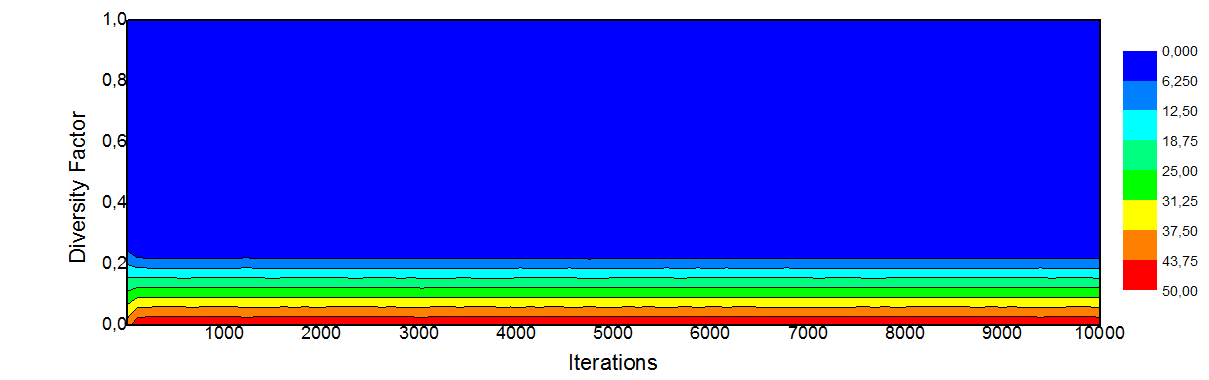
\includegraphics[scale=0.42]{results/diversity/ABPSO/F1/ABPSOF1.png}\label{fig:Diversity_ABPSO_F1_Factor}}
%\hspace{1mm}
%\subfigure[]{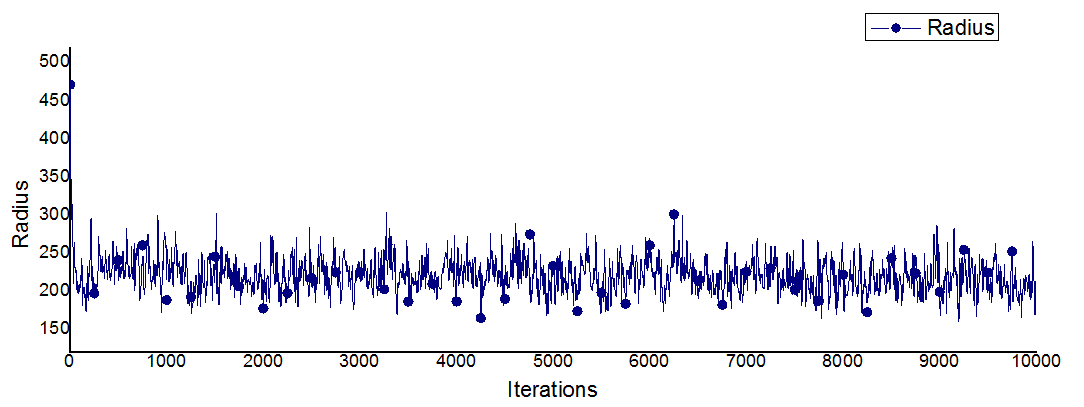
\includegraphics[scale=0.4]{results/diversity/ABPSO/F1/Radius.png}\label{fig:Diversity_ABPSO_F1_Radius}}
%\hspace{1mm}
%\subfigure[]{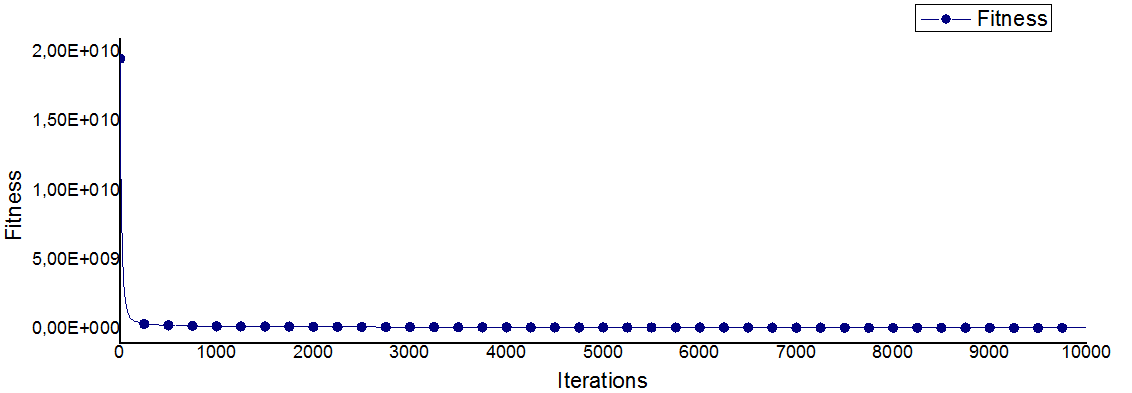
\includegraphics[scale=0.42]{results//diversity/ABPSO/F1/Fitness.png}\label{fig:Diversity_ABPSO_F1_Fitness}}
%\caption{\small{The evaluation of diversity of swarm for ABPSO algorithm: (a) diversity factor value, (b) radius value and (c) fitness value.}}
%\label{fig:Diversity_ABPSO_F1}
%\end{figure}
%
%The Figure \ref{fig:Diversity_ABC_F1} presents the results for ABC algorithm. The Figure \ref{fig:Diversity_ABC_F1_Factor} presents the behavior of the swarm, according to the diversity factor. One can see a expressive diversity generated by scout bees, when they find new food sources. In the Figure \ref{fig:Diversity_ABC_F1_Radius}, there is a variation of radius value of the swarm, but the radius value is high, so the swarm does not have a strong convergence capability. As explained before, the variation of radius value is because the scout bees. In the Figure \ref{fig:Diversity_ABC_F1_Fitness}, we can see the fitness value along of iterations and the limited convergence ability of algorithm, mainly if compared with the result of ABPSO algorithm.
%
%\begin{figure}[h]
%\centering
%\subfigure[]{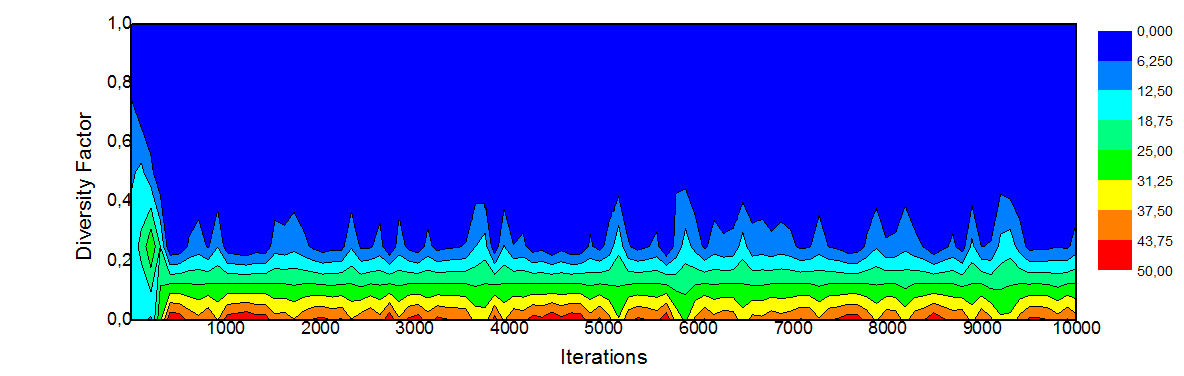
\includegraphics[scale=0.45]{results/diversity/ABC/F1/ABCF1.png}\label{fig:Diversity_ABC_F1_Factor}}
%\hspace{1mm}
%\subfigure[]{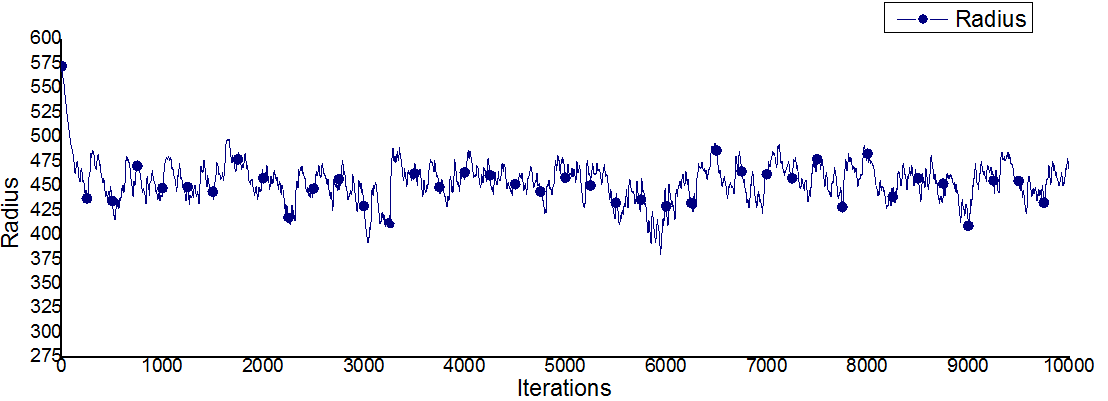
\includegraphics[scale=0.4]{results/diversity/ABC/F1/Radius.png}\label{fig:Diversity_ABC_F1_Radius}}
%\hspace{1mm}
%\subfigure[]{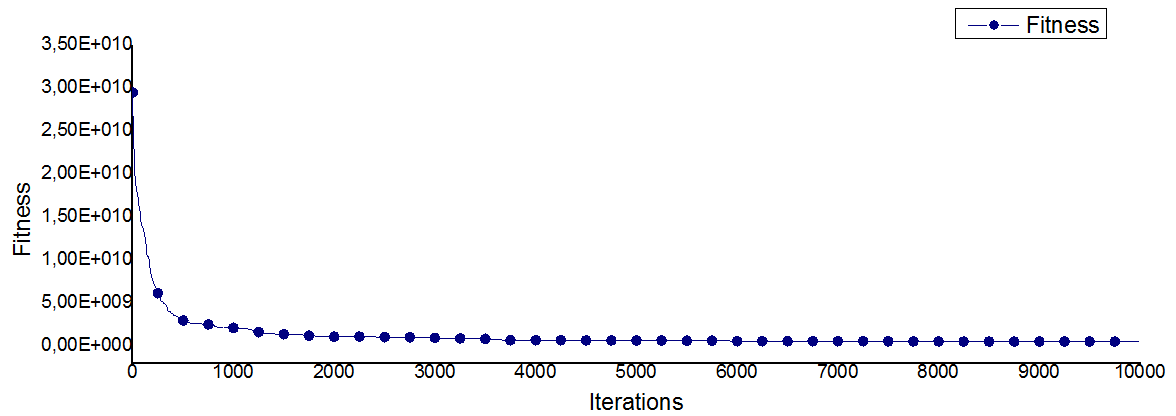
\includegraphics[scale=0.4]{results//diversity/ABC/F1/Fitness.png}\label{fig:Diversity_ABC_F1_Fitness}}
%\caption{\small{The evaluation of diversity of swarm for ABC algorithm: (a) diversity factor value, (b) radius value and (c) fitness value.}}
%\label{fig:Diversity_ABC_F1}
%\end{figure}
%
%The Figure \ref{fig:Diversity_PSO_F1} presents the results for PSO algorithm. The Figure \ref{fig:Diversity_PSO_F1_Factor} presents the behavior of the swarm, according to the diversity factor. One cannot see a significant diversity, because the algorithm does not have a mechanism to generate diversity, but the local communication topology helps to avoid a premature convergence of swarm. In the Figure \ref{fig:Diversity_PSO_F1_Radius}, there is a variation of radius value of the swarm, one can observe that the variation is low and the values is decreasing, this means that the swarm is contracting. In the Figure \ref{fig:Diversity_PSO_F1_Fitness}, we can see the fitness value along of iterations. Because of contraction state of swarm the algorithm has a good convergence ability.
%\begin{figure}[h]
%\centering
%\subfigure[]{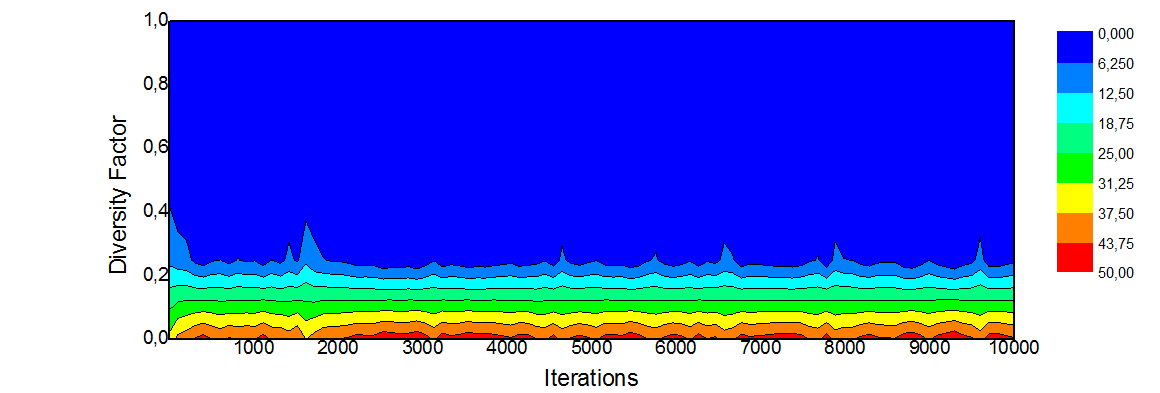
\includegraphics[scale=0.45]{results/diversity/PSO/F1/PSOF1.png}\label{fig:Diversity_PSO_F1_Factor}}
%\hspace{1mm}
%\subfigure[]{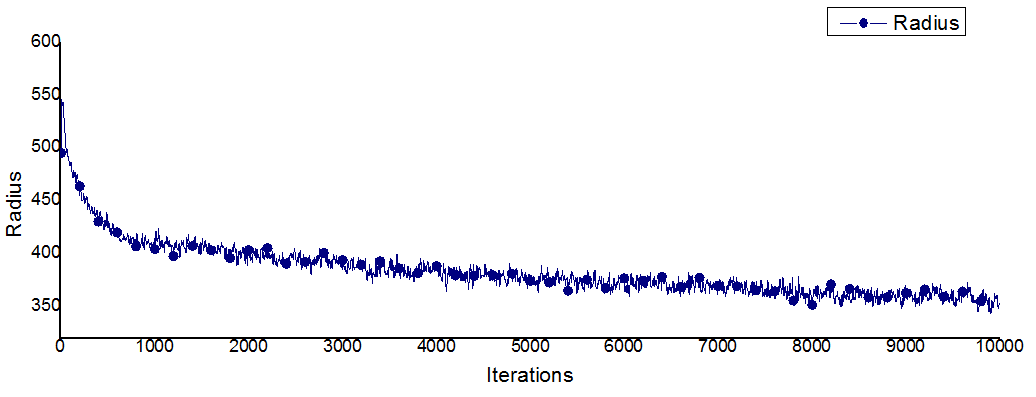
\includegraphics[scale=0.4]{results/diversity/PSO/F1/Radius.png}\label{fig:Diversity_PSO_F1_Radius}}
%\hspace{1mm}
%\subfigure[]{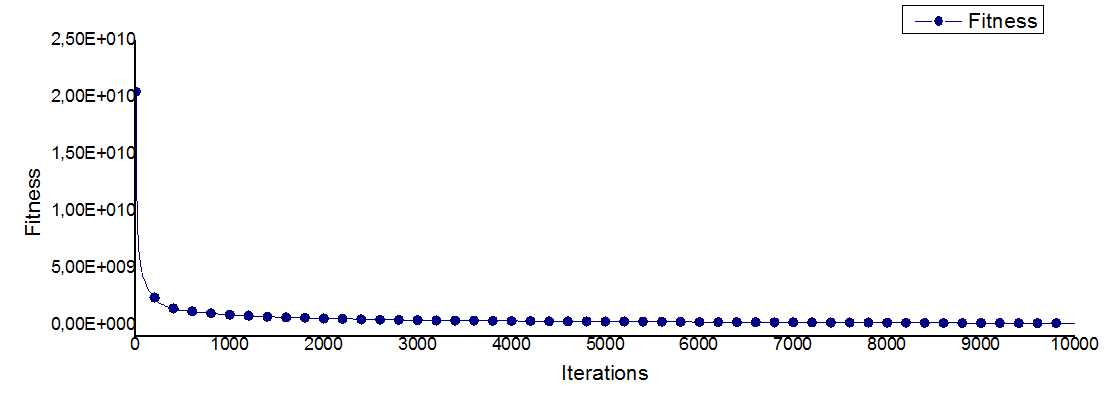
\includegraphics[scale=0.42]{results//diversity/PSO/F1/Fitness.png}\label{fig:Diversity_PSO_F1_Fitness}}
%\caption{\small{The evaluation of diversity of swarm for PSO algorithm: (a) diversity factor value, (b) radius value and (c) fitness value.}}
%\label{fig:Diversity_PSO_F1}
%\end{figure}
%
%The Figure \ref{fig:Diversity_FSS1_F1} presents the results for FSS algorithm, scenario 1. The Figure \ref{fig:Diversity_FSS1_F1_Factor} presents the behavior of the swarm, according to the diversity factor. One can observe the maintain of diversity, through the execution of collective-volitive movement that expand the school.  In the Figure \ref{fig:Diversity_FSS1_F1_Radius}, there is a variation of radius value of the swarm. We can see the contraction of swarm because the radius value decreased, however the variation is small because the volitive step value is small (this value is the double of individual step), consequently there is not expansion. In the Figure \ref{fig:Diversity_FSS1_F1_Fitness}, we can see the fitness value along of iterations. The maintain of diversity has consequences, the algorithm does not have a good convergence ability.
%\begin{figure}[h]
%\centering
%\subfigure[]{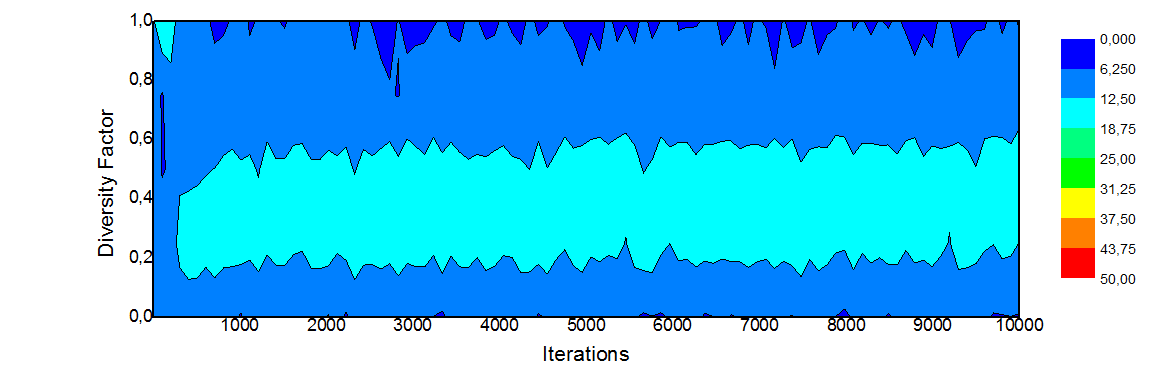
\includegraphics[scale=0.45]{results/diversity/FSS1/F1/FSSF1.png}\label{fig:Diversity_FSS1_F1_Factor}}
%\hspace{1mm}
%\subfigure[]{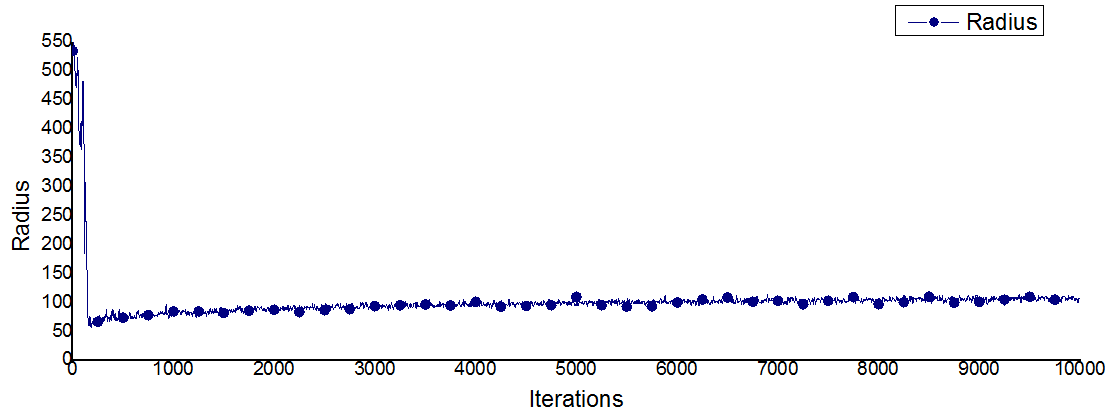
\includegraphics[scale=0.4]{results/diversity/FSS1/F1/Radius.png}\label{fig:Diversity_FSS1_F1_Radius}}
%\hspace{1mm}
%\subfigure[]{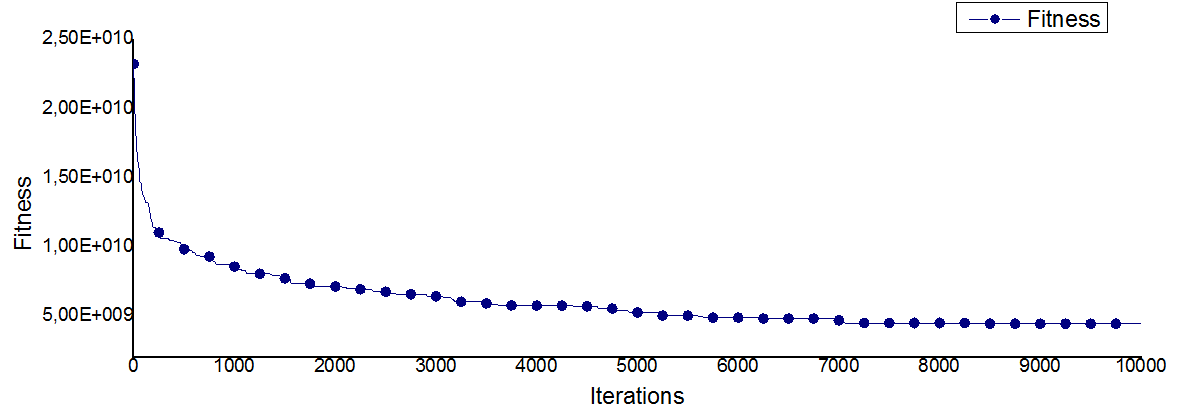
\includegraphics[scale=0.4]{results//diversity/FSS1/F1/Fitness.png}\label{fig:Diversity_FSS1_F1_Fitness}}
%\caption{\small{The evaluation of diversity of swarm for FSS algorithm scenario 1: (a) diversity factor value, (b) radius value and (c) fitness value.}}
%\label{fig:Diversity_FSS1_F1}
%\end{figure}
%
%The Figure \ref{fig:Diversity_FSS2_F1} presents the results for FSS algorithm, scenario 2. The Figure \ref{fig:Diversity_FSS2_F1_Factor} presents the behavior of the swarm, according to the diversity factor. One can observe the maintain of diversity, through the execution of collective-volitive movement that expand the school, but with the variation greater than scenario 1.  In the Figure \ref{fig:Diversity_FSS2_F1_Radius}, there is a variation of radius value of the swarm. We can see the contraction of swarm because the radius value decreased. As this scenario has the range values greater than scenario 1, there is a significant variation of radius value, but until a determined number of iterations. In the Figure \ref{fig:Diversity_FSS2_F1_Fitness}, we can see the fitness value along of iterations. Differently of the scenario 1, a big individual step value improve the convergence ability. When we compare the results of scenario 1 with scenario 2, the convergence speed of scenario 2 is better.
%\begin{figure}[h]
%\centering
%\subfigure[]{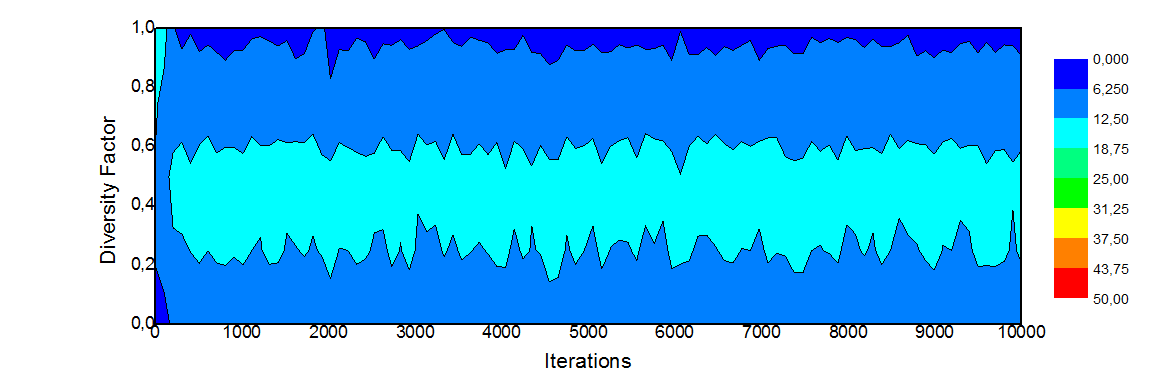
\includegraphics[scale=0.45]{results/diversity/FSS2/F1/FSSF1.png}\label{fig:Diversity_FSS2_F1_Factor}}
%\hspace{1mm}
%\subfigure[]{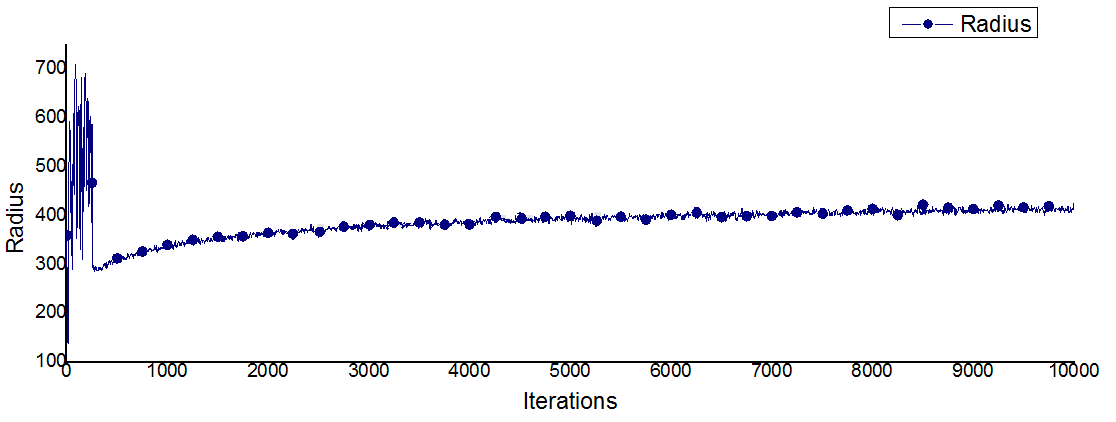
\includegraphics[scale=0.4]{results/diversity/FSS2/F1/Radius.png}\label{fig:Diversity_FSS2_F1_Radius}}
%\hspace{1mm}
%\subfigure[]{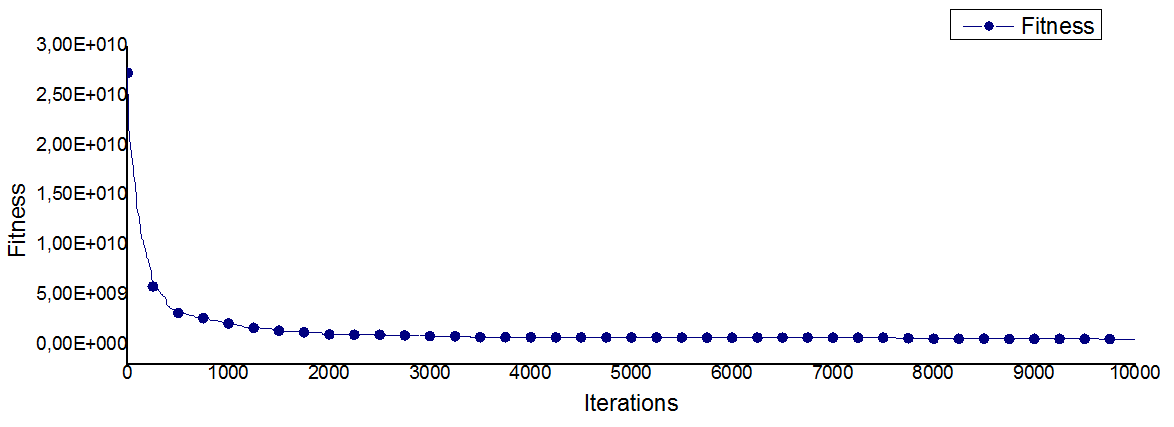
\includegraphics[scale=0.4]{results//diversity/FSS2/F1/Fitness.png}\label{fig:Diversity_FSS2_F1_Fitness}}
%\caption{\small{The evaluation of diversity of swarm for FSS algorithm scenario 2: (a) diversity factor value, (b) radius value and (c) fitness value.}}
%\label{fig:Diversity_FSS2_F1}
%\end{figure}

\section{Initial Analysis of the ClanABeePSO Algorithm}
This initial analysis shows the comparison of performance of ClanABeePSO with the ClanAPSO and ClanPSO algorithms. We used 100 dimensions and 1,000 iterations. This analysis was realized in five functions, the unimodal functions $F4$, $F7$ and $F19$, and the multimodal functions $F2$ and $F16$. We selected these functions in order to represent all classes of problems described in the entire benchmark.

In the conference of leaders, we executed the PSO algorithm and we tested two communication topologies, local and global. We adopted the following nomenclature for the ClanABeePSO based algorithms: ``$<$Name of algorithm$>$ - L'' means the local communication topology  and ``$<$Name of algorithm$>$- G'', global topology.

Table \ref{tab:ClanABeePSO_Local} presents the average fitness and (standard deviation) for local topology. One can observe that, in the most of cases, our proposal achieved better results than other techniques (the exception is $F2$ function). According to Table \ref{tab:ClanABeePSO_Global}, we can conclude the same for the global topology. One can observe that the local topology achieved the best results in most of cases when compared to the global topology. %But, the different is small, so it is necessary to make a deeper analysis, with statistical tests.


\begin{table}[!h]
\caption{\small{Comparison of ClanABeePSO, ClanAPSO and ClanPSO algorithms with conference of leaders executing a Local PSO.}}
\centering
\begin{tabular}{p{0.5cm}|p{3.0cm}|p{3.0cm}|p{3.0cm}}
\hline
\textbf{F\#}  & ClanABeePSO - L &  ClanAPSO - L & ClanPSO - L \\
\hline
$F2$      &  1031.6137 (56.0135) &  \textbf{771.6618 (101.8197)}   &  1249.418 (61.9373) \\
$F4$      &  \textbf{1.56E+14 (4.1E+13)}  &  2.66E+14 (1.04E+04)   &  4.97E+14 (1.62E+14) \\
$F7$      &  \textbf{3.99E+10 (1.06E+10)} &  7.34E+10 (1.44E+10)   &  8.87E+10 (1.86E+10) \\
$F16$     &  \textbf{30.1947 (1.5911)}    &  39.5529  (0.8987)     &  40.6395 (0.27026) \\
$F19$     &  \textbf{2.18E+05 (2.85E+04)} &  3.03E+05 (6.91E+04)   &  3.56E+05 (6.01E+04)\\
\hline
\end{tabular}
\label{tab:ClanABeePSO_Local}
\end{table}

\begin{table}[!h]
\caption{\small{Comparison of ClanABeePSO, ClanAPSO and ClanPSO algorithms with conference of leaders executing a global PSO.}}
\centering
\begin{tabular}{p{0.5cm}|p{3.0cm}|p{3.0cm}|p{3.0cm}}
\hline
\textbf{F\#}  & ClanABeePSO - G &  ClanAPSO - G & ClanPSO - G\\
\hline
$F2$      &   1026.3147 (58.1114)   &  \textbf{838.1519 (71.2261)}   & 1291.227 (64.2355) \\
$F4$      &   \textbf{1.65E+04 (3.54E+13)}   &  2.87E+14 (1.00E+14)  & 4.99E+14 (1.94E+14) \\
$F7$      &   \textbf{3.85E+10 (6.81E+09)}   &  8.58E+10 (1.82E+10)    & 9.61E+10 (2.11E+10) \\
$F16$     &   \textbf{30.3466 (1.5815)}      &  39.6915 (0.6011)     &  40.7952 (0.3673)\\
$F19$     &   \textbf{2.29E+05 (3.57E+04)}   &  3.32E+05 (7.83E+04)  & 3.39E+05 (8.67E+04) \\
\hline
\end{tabular}
\label{tab:ClanABeePSO_Global}
\end{table}

We also performed an analysis executing the APSO algorithm in the conference of leaders. We tested in all benchmark functions.
Table \ref{tab:Comparison_ClanABeePSO_PSO} presents the results with the use the PSO algorithm in conference of leaders. The results for the PSO algorithm used in the conference of leaders are better than when the APSO algorithm is used (observe table \ref{tab:Comparison_ClanABeePSO_APSO}). For the unimodal functions, the ClanABeePSO achieved better results than the ClanAPSO. For the multimodal functions, the ClanABeePSO algorithm did not achieved the desired performance for the Rastrigin-based functions ($F2$, $F5$, $F10$ and $F15$).

\begin{table}[!h]
\caption{\small{Performance comparison in terms of average fitness value and (standard deviation) between ClanABeePSO and ClaAPSO with execution of PSO in the conference of leaders for all the 20 benchmark functions for 100 dimensions.}}
\label{tab:Comparison_ClanABeePSO_PSO}
\begin{center}
\begin{tabular}{p{0.5cm}|p{2.5cm}|p{2.5cm}|p{2.5cm}|p{2.5cm}}
\hline\noalign{\smallskip}
\textbf{F\#}	& ClanABeePSO - L & ClanABeePSO - G & ClanAPSO - L & ClanAPSO - G    \\		
\noalign{\smallskip}
\hline
\noalign{\smallskip}
\textit{F1}  & 5.45E+08 (1.08E+08)& \textbf{5.29E+08 (1.33E+08)} & 2.61E+09 (1.14E+09) & 2.42E+09 (1.03E+09)\\
\textit{F2}  & 1031.6137 (56.0135) & 1026.3147 (58.1114) & \textbf{771.6618 (101.8197)} & 838.1519 (71.2261)\\
\textit{F3}  & 13.1624 (0.5596) & \textbf{12.5989 (0.4668)} & 19.0352 (0.6809) & 19.3434 (0.5242)\\
\textit{F4}  & \textbf{1.56E+14 (4.1E+13)} & 1.65E+14 (3.54E+13) & 2.66E+14 (1.04E+14) & 2.87E+14 (1.00E+14)\\
\textit{F5}  & 4.2E+08 (2.35E+07) & 4.17E+08 (2.48E+07) & \textbf{3.50E+08 (4.72E+07)} & 3.92E+08 (4.79E+07)\\
\textit{F6}  & 1.04E+07 (8.58E+05) & \textbf{9.41E+06 (5.57E+05)} & 1.87E+07 (9.67E+05) & 1.89E+07 (8.04E+05)\\
\textit{F7}  & 3.99E+10 (1.06E+10) & \textbf{3.85E+10 (6.81E+09)} & 7.34E+10 (1.44E+10) & 8.58E+10 (1.82E+10)\\
\textit{F8}  & 1.14E+14 (7.28E+13) & \textbf{7.22E+13 (2.33E+13)} & 2.09E+16 (9.78E+15) & 2.32E+16 (1.05E+16)\\
\textit{F9}  & 7.62E+08 (2.51E+08) & \textbf{5.8E+08 (1.07E+08)} & 1.11E+09 (5.34E+08) & 1.64E+09 (5.92E+08)\\
\textit{F10} & 1050.3797 (52.3948) & 1021.8675 (51.4933) & \textbf{704.9859 (87.0795)} & 930.2839 (83.4512)\\
\textit{F11} & 29.8896 (1.8033) & \textbf{29.5806 (1.6640)} & 37.6465 (1.3326) & 38.5982 (0.8247)\\
\textit{F12} & \textbf{7.77E+04 (9.97E+03)} & 1.04E+05 (2.09E+04) & 2.59E+05 (4.19E+04) & 2.73E+05 (4.84E+04)\\
\textit{F13} & \textbf{8.12E+07 (2.12E+07)} & 1.29E+08 (1.09E+08) & 1.61E+10 (5.28E+09) & 1.58E+10 (6.89E+09)\\
\textit{F14} & \textbf{8.09E+08 (1.3E+08)} & 8.52E+08 (1.45E+08) & 1.14E+09 (3.50E+08) & 1.18E+09 (3.73E+08)\\
\textit{F15} & 1070.2954 (48.2117) & 1067.4445 (53.4160) & \textbf{988.4879 (79.7370)} & 1012.5407 (79.9971)\\
\textit{F16} & \textbf{30.1947 (1.5911)} & 30.3466 (1.5815) & 39.5529 (0.8987) & 39.6915 (0.6011)\\
\textit{F17} & \textbf{1.91E+05 (2.50E+04)} & 2.08E+05 (3.21E+04) & 2.65E+05 (5.46E+04) & 2.70E+05 (4.30E+04)\\
\textit{F18} & \textbf{8.92E+08 (1.9E+08)} & 1.25E+09 (5.44E+08) & 7.83E+10 (1.65E+10) & 7.61E+10 (1.46E+10)\\
\textit{F19} & \textbf{2.18E+05 (2.85E+04)} & 2.29E+05 (3.57E+04) & 3.03E+05 (6.91E+04) & 3.32E+05 (7.83E+04)\\
\textit{F20} & \textbf{7.07E+08 (1.59E+08)} & 1.19E+09 (6.34E+08) & 1.04E+11 (2.04E+10) & 1.00E+11 (2.19E+10)\\
\hline
\end{tabular}
\end{center}
\end{table}

\begin{table}[!h]
\caption{\small{Performance comparison in terms of average fitness value and (standard deviation) between ClanABeePSO and ClaAPSO with execution of APSO in the conference of leaders for all the 20 benchmark functions for 100 dimensions.}}
\label{tab:Comparison_ClanABeePSO_APSO}
\begin{center}
\begin{tabular}{p{0.5cm}|p{2.5cm}|p{2.5cm}|p{2.5cm}|p{2.5cm}}
\hline\noalign{\smallskip}
\textbf{F\#}	& ClanABeePSO - L & ClanABeePSO - G & ClanAPSO - L & ClanAPSO - G \\		
\noalign{\smallskip}
\hline
\noalign{\smallskip}
\textit{F1}  & \textbf{2.14E+09 (8.18E+08)} & 2.21E+09 (8.77E+08) & 3.56E+09 (1.38E+09) & 3.33E+09 (1.29E+09)\\
\textit{F2}  & \textbf{818.9345 (62.1110)} & 854.3629 (72.2428) & 833.5397 (80.1530) & 845.7962 (88.5562)\\
\textit{F3}  & 19.5079 (0.3109) & 19.5476 (0.2776) & \textbf{19.4254 (0.3693)} & 19.4973 (0.3233)\\
\textit{F4}  & \textbf{2.21E+14 (9.49E+13)} & 2.5E+14 (9.76E+13) & 3.84E+14 (1.52E+14) & 4.12E+14 (1.79E+14)\\
\textit{F5}  & \textbf{3.85E+08 (5.14E+07)} & 3.97E+08 (5.20E+07) & 4.14E+08 (5.72E+07) & 4.11E+08 (5.47E+07)\\
\textit{F6}  & \textbf{1.94E+07 (3.89E+05)} & 1.95E+07 (3.28E+05) & 1.95E+07 (3.34E+05) & 1.96E+07 (3.54E+05)\\
\textit{F7}  & \textbf{7.6E+10 (1.63E+10)} & 8.07E+10 (1.68E+10) & 9.69E+10 (1.97E+10) & 1.01E+11 (2.69E+10)\\
\textit{F8}  & 2.16E+16 (9.48E+15) & \textbf{2.14E+16 (8.29E+15)} & 3.14E+16 (1.21E+16) & 2.93E+16 (8.79E+15)\\
\textit{F9}  & 1.58E+09 (5.22E+08) & \textbf{1.53E+09 (4.9E+08)} & 2.82E+09 (1.08E+09) & 2.47E+09 (6.68E+08)\\
\textit{F10} & 914.0123 (105.0599) & 936.1181 (95.7550) & \textbf{887.2911 (113.8297)} & 928.4704 (82.8355)\\
\textit{F11} & 38.8131 (0.8369) & 38.7006 (0.7980) & \textbf{38.3081 (1.0786)} & 38.7691 (0.7347)\\
\textit{F12} & \textbf{2.51E+05 (3.72E+04)} & 2.59E+05 (4.30E+04) & 3.14E+05 (4.55E+04) & 3.48E+05 (5.33E+04)\\
\textit{F13} & 1.38E+10 (5.15E+09) & \textbf{1.27E+10 (4.36E+09)} & 1.95E+10 (6.57E+09) & 1.94E+10 (5.98E+09)\\
\textit{F14} & \textbf{1.09E+09 (3.73E+08)} & 1.24E+09 (3.48E+08) & 1.28E+09 (4.40E+08) & 1.54E+09 (4.73E+08)\\
\textit{F15} & 1026.1148 (67.3962) & 1043.2662 (90.3853) & \textbf{1019.0113 (70.6286)} & 1025.8771 (91.8249)\\
\textit{F16} & 39.8903 (0.3489) & \textbf{39.6015 (0.3553)} & 39.7034 (0.3414) & 39.7101 (0.4693)\\
\textit{F17} & 2.72E+05 (4.79E+04) & \textbf{2.62E+05 (4.61E+04)} & 3.26E+05 (6.58E+04) & 3.19E+05 (7.37E+04)\\
\textit{F18} & 7.49E+10 (1.36E+10) & \textbf{7.19E+10 (1.37E+10)} & 8.24E+10 (1.46E+10) & 8.47E+10 (1.27E+10)\\
\textit{F19} & \textbf{3.02E+05 (6.55E+04)} & 3.12E+05 (6.05E+04) & 3.75E+05 (9.05E+04) & 3.82E+05 (8.33E+04)\\
\textit{F20} & 1.08E+11 (2.14E+10) & \textbf{1.02E+11 (1.82E+10)} & 1.19E+11 (2.23E+10) & 1.19E+11 (1.85E+10)\\
\hline
\end{tabular}
\end{center}
\end{table}

%\begin{table}[!h]
%\caption{\small{Performance comparison in terms of average fitness value and (standard deviation) between ClanABPSO and ClaAPSO with execution of PSO }}
%%in the conference of leaders for all the 20 benchmark functions for 100 dimensions.
%\label{tab:Comparison_ClanABPSO_PSO}
%\begin{center}
%\begin{tabular}{p{0.5cm}|p{2.1cm}|p{2.1cm}|p{2.1cm}|p{2.1cm}|p{2.1cm}}
%\hline\noalign{\smallskip}
%\textbf{F\#}	& ABPSO & ClanABPSO - L & ClanABPSO - G & ClanAPSO - L & ClanAPSO - G    \\		
%\noalign{\smallskip}
%\hline
%\noalign{\smallskip}
%\textit{F1}  & \textbf{2.86E+08 (8.22E+07)} & 5.45E+08 (1.08E+08)& 5.29E+08 (1.33E+08) & 2.61E+09 (1.14E+09) & 2.42E+09 (1.03E+09)\\
%\textit{F2}  & 958.6346 (63.09667) & 1031.6137 (56.0135) & 1026.3147 (58.1114) & \textbf{771.6618 (101.8197)} & 838.1519 (71.2261)\\
%\textit{F3}  & \textbf{12.07975 (0.656529)} & 13.1624 (0.5596) & 12.5989 (0.4668) & 19.0352 (0.6809) & 19.3434 (0.5242)\\
%\textit{F4}  & \textbf{1.32E+14 (3.05E+13)} & 1.56E+14 (4.1E+13) & 1.65E+14 (3.54E+13) & 2.66E+14 (1.04E+14) & 2.87E+14 (1.00E+14)\\
%\textit{F5}  & 3.81E+08 (2.64E+07) & 4.2E+08 (2.35E+07) & 4.17E+08 (2.48E+07) & \textbf{3.50E+08 (4.72E+07)} & 3.92E+08 (4.79E+07)\\
%\textit{F6}  & \textbf{7.59E+06 (8.71E+05)} & 1.04E+07 (8.58E+05) & 9.41E+06 (5.57E+05) & 1.87E+07 (9.67E+05) & 1.89E+07 (8.04E+05)\\
%\textit{F7}  & 4.33E+10 (9.10E+09) & 3.99E+10 (1.06E+10) & \textbf{3.85E+10 (6.81E+09)} & 7.34E+10 (1.44E+10) & 8.58E+10 (1.82E+10)\\
%\textit{F8}  & \textbf{6.78E+13 (5.49E+05)} & 1.14E+14 (7.28E+13) & 7.22E+13 (2.33E+13) & 2.09E+16 (9.78E+15) & 2.32E+16 (1.05E+16)\\
%\textit{F9}  & \textbf{4.02E+08 (9.68E+07)} & 7.62E+08 (2.51E+08) & 5.8E+08 (1.07E+08) & 1.11E+09 (5.34E+08) & 1.64E+09 (5.92E+08)\\
%\textit{F10} & 973.3662 (39.8397) & 1050.3797 (52.3948) & 1021.8675 (51.4933) & \textbf{704.9859 (87.0795)} & 930.2839 (83.4512)\\
%\textit{F11} & \textbf{25.93234 (2.34576)} & 29.8896 (1.8033) & 29.5806 (1.6640) & 37.6465 (1.3326) & 38.5982 (0.8247)\\
%\textit{F12} & 9.26E+04 (1.67E+04) & \textbf{7.77E+04 (9.97E+03)} & 1.04E+05 (2.09E+04) & 2.59E+05 (4.19E+04) & 2.73E+05 (4.84E+04)\\
%\textit{F13} & \textbf{8.08E+07 (7.19E+07)} & 8.12E+07 (2.12E+07) & 1.29E+08 (1.09E+08) & 1.61E+10 (5.28E+09) & 1.58E+10 (6.89E+09)\\
%\textit{F14} & \textbf{6.29E+08 (1.21E+08)} & 8.09E+08 (1.3E+08) & 8.52E+08 (1.45E+08) & 1.14E+09 (3.50E+08) & 1.18E+09 (3.73E+08)\\
%\textit{F15} & \textbf{982.0151 (40.05412)} & 1070.2954 (48.2117) & 1067.4445 (53.4160) & 988.4879 (79.7370) & 1012.5407 (79.9971)\\
%\textit{F16} & \textbf{25.48114 (2.66121)} & 30.1947 (1.5911) & 30.3466 (1.5815) & 39.5529 (0.8987) & 39.6915 (0.6011)\\
%\textit{F17} & \textbf{1.84E+05 (2.29E+04)} & 1.91E+05 (2.50E+04) & 2.08E+05 (3.21E+04) & 2.65E+05 (5.46E+04) & 2.70E+05 (4.30E+04)\\
%\textit{F18} & 1.02E+09 (6.82E+08) & \textbf{8.92E+08 (1.9E+08)} & 1.25E+09 (5.44E+08) & 7.83E+10 (1.65E+10) & 7.61E+10 (1.46E+10)\\
%\textit{F19} & \textbf{2.09E+05 (2.82E+04)} & 2.18E+05 (2.85E+04) & 2.29E+05 (3.57E+04) & 3.03E+05 (6.91E+04) & 3.32E+05 (7.83E+04)\\
%\textit{F20} & 1.09E+09 (6.41E+08) & \textbf{7.07E+08 (1.59E+08)} & 1.19E+09 (6.34E+08) & 1.04E+11 (2.04E+10) & 1.00E+11 (2.19E+10)\\
%\hline
%\end{tabular}
%\end{center}
%\end{table}
%
%\begin{table}[!h]
%\caption{\small{Performance comparison in terms of average fitness value and (standard deviation) between ClanABPSO and ClaAPSO with execution of APSO}}
%%in the conference of leaders for all the 20 benchmark functions for 100 dimensions.
%\label{tab:Comparison_ClanABPSO_APSO}
%\begin{center}
%\begin{tabular}{p{0.5cm}|p{2.1cm}|p{2.1cm}|p{2.1cm}|p{2.1cm}|p{2.1cm}}
%\hline\noalign{\smallskip}
%\textbf{F\#}	& ABPSO & ClanABPSO - L & ClanABPSO - G & ClanAPSO - L & ClanAPSO - G \\		
%\noalign{\smallskip}
%\hline
%\noalign{\smallskip}
%\textit{F1} & \textbf{2.86E+08 (8.22E+07)}  & 2.14E+09 (8.18E+08) & 2.21E+09 (8.77E+08) & 3.56E+09 (1.38E+09) & 3.33E+09 (1.29E+09)\\
%\textit{F2} & 958.6346 (63.09667) & \textbf{818.9345 (62.1110)} & 854.3629 (72.2428) & 833.5397 (80.1530) & 845.7962 (88.5562)\\
%\textit{F3} & \textbf{12.07975 (0.656529)} & 19.5079 (0.3109) & 19.5476 (0.2776) & 19.4254 (0.3693) & 19.4973 (0.3233)\\
%\textit{F4} & \textbf{1.32E+14 (3.05E+13)} & 2.21E+14 (9.49E+13) & 2.5E+14 (9.76E+13) & 3.84E+14 (1.52E+14) & 4.12E+14 (1.79E+14)\\
%\textit{F5} & \textbf{3.81E+08 (2.64E+07)} & 3.85E+08 (5.14E+07) & 3.97E+08 (5.20E+07) & 4.14E+08 (5.72E+07) & 4.11E+08 (5.47E+07)\\
%\textit{F6}  & \textbf{7.59E+06 (8.71E+05)} & 1.94E+07 (3.89E+05) & 1.95E+07 (3.28E+05) & 1.95E+07 (3.34E+05) & 1.96E+07 (3.54E+05)\\
%\textit{F7} & \textbf{4.33E+10 (9.10E+09)} & 7.6E+10 (1.63E+10) & 8.07E+10 (1.68E+10) & 9.69E+10 (1.97E+10) & 1.01E+11 (2.69E+10)\\
%\textit{F8}  & \textbf{6.78E+13 (5.49E+05)} & 2.16E+16 (9.48E+15) & 2.14E+16 (8.29E+15) & 3.14E+16 (1.21E+16) & 2.93E+16 (8.79E+15)\\
%\textit{F9} & \textbf{4.02E+08 (9.68E+07)} & 1.58E+09 (5.22E+08) & 1.53E+09 (4.9E+08) & 2.82E+09 (1.08E+09) & 2.47E+09 (6.68E+08)\\
%\textit{F10} & 973.3662 (39.8397) & 914.0123 (105.0599) & 936.1181 (95.7550) & \textbf{887.2911 (113.8297)} & 928.4704 (82.8355)\\
%\textit{F11} & \textbf{25.93234 (2.34576)} & 38.8131 (0.8369) & 38.7006 (0.7980) & 38.3081 (1.0786) & 38.7691 (0.7347)\\
%\textit{F12} & \textbf{9.26E+04 (1.67E+04)} & 2.51E+05 (3.72E+04) & 2.59E+05 (4.30E+04) & 3.14E+05 (4.55E+04) & 3.48E+05 (5.33E+04)\\
%\textit{F13} & \textbf{8.08E+07 (7.19E+07)} & 1.38E+10 (5.15E+09) & 1.27E+10 (4.36E+09) & 1.95E+10 (6.57E+09) & 1.94E+10 (5.98E+09)\\
%\textit{F14} & \textbf{6.29E+08 (1.21E+08)} & 1.09E+09 (3.73E+08) & 1.24E+09 (3.48E+08) & 1.28E+09 (4.40E+08) & 1.54E+09 (4.73E+08)\\
%\textit{F15} & \textbf{982.0151 (40.05412)} & 1026.1148 (67.3962) & 1043.2662 (90.3853) & 1019.0113 (70.6286) & 1025.8771 (91.8249)\\
%\textit{F16} & \textbf{25.48114 (2.66121)} & 39.8903 (0.3489) & 39.6015 (0.3553) & 39.7034 (0.3414) & 39.7101 (0.4693)\\
%\textit{F17} & \textbf{1.84E+05 (2.29E+04)} & 2.72E+05 (4.79E+04) & 2.62E+05 (4.61E+04) & 3.26E+05 (6.58E+04) & 3.19E+05 (7.37E+04)\\
%\textit{F18} & \textbf{1.02E+09 (6.82E+08)} & 7.49E+10 (1.36E+10) & 7.19E+10 (1.37E+10) & 8.24E+10 (1.46E+10) & 8.47E+10 (1.27E+10)\\
%\textit{F19} & \textbf{2.09E+05 (2.82E+04)} & 3.02E+05 (6.55E+04) & 3.12E+05 (6.05E+04) & 3.75E+05 (9.05E+04) & 3.82E+05 (8.33E+04)\\
%\textit{F20} & \textbf{1.09E+09 (6.41E+08)} & 1.08E+11 (2.14E+10) & 1.02E+11 (1.82E+10) & 1.19E+11 (2.23E+10) & 1.19E+11 (1.85E+10)\\
%\hline
%\end{tabular}
%\end{center}
%\end{table}

\pagebreak
